%%%%%%%%%%%%%%%%%%%%%%%%%%%%%%%%%%%%%%%%%
% MODELE DE MANUSCRIT DE THESE 
% DE L'UNIVERSITE PARIS CITE
% OFFICIEL

% LaTeX Template
% Version overleaf (14/10/2023) 
% Format BOOK
% Par Aleksandra SAVINA, PhD
% https://www.overleaf.com/latex/templates/phd-thesis-template-universite-paris-cite/jycfrbbjbgrm
%%%%%%%%%%%%%%%%%%%%%%%%%%%%%%%%%%%%%%%%%


%----------------------------------------------------------------------------------------
%	PREAMBULE // PACKAGES AND OTHER DOCUMENT CONFIGURATIONS
%----------------------------------------------------------------------------------------

\documentclass[a4paper,12pt,twoside,french]{book}
\usepackage{PackagesDeAmbroise}
\addbibresource{biblio_ESH.bib}
\addbibresource{Mémoire_ESH.bib}
\addbibresource{Mémoire_ESH2.bib}


\selectlanguage{french}%
\linespread{1.2} % Line spacing of 1.5 times the normal spacing
\title{Memoire M2 ESH}
\author{Ambroise Warnery}
\date{October 2024}

% Headers footers and glossaires
\fancyhead{} % clear all header fields
\fancyfoot{} % clear all footer fields
\fancyfoot[RO,LE]{\thepage}  % fait apparaitre les numéros de page en bas à l'exterieur
\setlength{\headheight}{14.5pt}

% \makeglossaries
% \makeindex
%%%%%%%%%%%%%%%%%%%%%%%%%%%%%%%%%%%%%%%%%%%%%%%%%%%%%%%%%%%%%%%%%%%%%%%%%%
%%%%%%%%%%%%%%%%%%%%%%%%%%%%%%%%%%%%%%%%%%%%%%%%%%%%%%%%%%%%%%%%%%%%%%%%%%
%----------------------------------------------------------------------------------------
%	DOCUMENT
%----------------------------------------------------------------------------------------
\begin{document}


%\maketitle
%----------------------------------------------------------------------------------------
%	TITLE PAGE
%----------------------------------------------------------------------------------------
\begin{titlepage}
    \begin{center}
            
\includegraphics[height=2.5cm]{figures/cover/logoparis1.png}
    \end{center}

    \begin{center}
    
\vspace*{.03\textheight}
\textsc{\LARGE Université Paris-Panthéon-Sorbonne}\\[0.2cm] % Univ name
    \large M2 - ESH\\
          \vfill
            \rule{\textwidth}{0.8pt} \\ % Ligne horizontale
            \vspace{10pt}
            {\LARGE \bfseries Les programmeurs-économistes et leurs logiciels (1970-2010)}\\[0.4cm] % Titre principal
            {\large \itshape Une analyse de leurs parcours, de leurs pratiques et quelques perspectives sur l'avenir} % Sous-titre
            \vspace{10pt}
            \rule{\textwidth}{0.8pt} \\ % Ligne horizontale
    \end{center}
    
    \vfill
    % Author and supervisor	
    \begin{center}
        Par \textsc{\Large Ambroise WARNERY}\\[1cm] 
        Mémoire de recherche\\[1.2cm]
        Dirigé par \textsc{\large Francesco SERGI}\\[0.2cm]
        Présenté et soutenu le 10/09/2025 %renseigner la date et choisir le type de soutenance
    \end{center}
    
    \vspace{1cm}


\newpage %page de garde vide
\thispagestyle{empty} %page de garde vide
\end{titlepage}

\renewcommand{\chaptermark}[1]{\markboth{#1}{}}




% --------------------------------------------------------------
%                         Début du corps
% --------------------------------------------------------------

\mainmatter
\setlength{\parskip}{1.2em}

\renewcommand{\baselinestretch}{1.1} %interligne pour le texte standard

\fancyhead[RO]{\leftmark}
\fancyhead[LE]{\textsc{\chaptername~\thechapter}}

\tableofcontents

\chapter*{Introduction}
\addcontentsline{toc}{chapter}{Introduction}

Mary Morgan, dans son livre de 2012, The World in the Model: How Economists Work and Think\cite{morganWorldModel}, décrit l'économie comme une "science outillée", et analyse le rôle centrale des modèles. Un autre outil, moins souvent étudié, est devenu tout aussi structurant.

Il s'agit de l'outil informatique.

Depuis les années 1970, l’usage de l’informatique en économie n’a cessé de s'intensifier. Il s’impose aujourd’hui dans toutes les dimensions de la recherche : simulation, expérimentation, traitement de données ou encore modélisation basée agent. Derrière cette transformation technique, on trouve des trajectoires individuelles bien concrètes : celles des programmeurs-économistes, à la fois chercheurs et développeurs, dont les contributions ne se limitent pas à l’usage d’outils existants, mais incluent la création de logiciels devenus centraux dans certains sous-champs de la discipline (voir Boumans et al. 2023\cite{boumansComputerizationEconomicsThree2023}, Cherrier et al. 2023\cite{cherrierWriteYourModel2023}, Backhouse et al. 2017 \cite{backhouseItsComputersStupid2017}). 

Ce travail s’appuie sur une série d’entretiens réalisés dans le cadre du projet Oral Histories of Economics, avec 7 figures ayant contribué de manière significative à cette hybridation entre économie et informatique : David Hendry\cite{hendryInterviewDavidHendry2024}, Joshua Epstein\cite{epsteinInterviewJoshuaEpstein2024}, Robert Axtell\cite{axtellInterviewRobertAxtell2025}, Theodore Turocy\cite{turocyInterviewTheodoreTurocy2024}, Urs Fischbacher\cite{fischbacherInterviewUrsFischbacher2024}, Richard Pierse\cite{pierseInterviewRichardPierse2024} et Agnès Gramain\cite{gramainInterviewAgnesGramain2024}. À travers leurs récits, il s’agit de documenter, comparer et analyser leurs trajectoires, afin de mieux comprendre comment se forment, s’exercent et se diffusent les compétences de programmation en économie, quels types de profils les incarnent, et comment l'évolution de l'informatique influence les pratiques du programmeur-économiste. 

L’objectif de ce mémoire est double. Il s’agit de dresser un portrait des programmeurs-économistes et des logiciels qu’ils ont conçus, en identifiant à la fois leurs traits communs — modalités d’apprentissage de l’informatique, profils académiques hybrides, diversité des langages mobilisés, rapports de genre, confrontation aux contraintes techniques et institutionnelles — et leurs différences, qu’elles soient générationnelles, institutionnelles ou techniques.

Puis d'analyser ces spécificités. Il s’agira de les mettre en perspective, de les comparer aux évolutions récentes de l’informatique en économie, et d’interroger ce qu’elles révèlent du rôle de la programmation dans la production et la transformation des savoirs économiques.

Le mémoire se déploie trois chapitres. Le premier est consacré à l’analyse biographique des programmeurs-économistes rencontrés, afin de dégager leurs traits communs et leurs différences. Le deuxième s’attache aux logiciels qu’ils ont conçus : leurs objectifs, leurs usages et leurs devenirs. Le troisième propose une analyse de ces trajectoires.

Méthodologiquement, ce travail repose principalement sur l’analyse qualitative des entretiens, qui constituent des sources situées et construites. Comme le rappelle Jullien \cite{jullienInterviewsMethodologicalHistoriographical2018}, les récits oraux sont traversés par des enjeux de légitimité et par des choix narratifs. Ils doivent donc être lus avec précaution, en tenant compte des silences, des oublis et des stratégies discursives. Nous avons cherché à croiser ces témoignages avec d’autres sources (documents publics, littérature secondaire) afin d'en proposer une lecture réflexive et critique.



\chapter*{Methodologie}
\addcontentsline{toc}{chapter}{Méthodologie}

Ce mémoire utilise comme littérature primaire, au sens où ce sont les matériaux que l'on vise à analyser, une collection de 7 entretiens. Ce corpus se compose d’entretiens semi-directifs menés avec des économistes ayant participé au développement de logiciels ou ayant fait un usage intensif de l’informatique dans leur pratique scientifique. 7 trajectoires sont analysées : celles d’Agnès Gramain, Urs Fischbacher, David Hendry, Richard Pierse, Theodore Turocy, Joshua Epstein et Robert Axtell. La réflexion menée dans ce mémoire repose sur une analyse qualitative et comparative de ces entretiens. Nous nous appuierons également sur une analyse de la littérature secondaire, au sens de la recherche académique portant sur le même sujet, sur la documentation des logiciels et les logiciels dont il est question dans les entretiens, ainsi que notre parcours académique en tant qu'étudiant en économie, économétrie puis épistémologie, qui nous a permis d'expérimenter la programmation pour l'économie, qui nous a donné l'occasion de rencontrer et de discuter avec beaucoup d'étudiants, professeurs, chercheurs liés de près ou de loin à cette thématique.

Le corpus d'entretiens que nous analysons dans ce mémoire provient du projet \textit{Oral Histories of Economics}, coordonné par Francesco Sergi et Dorian Jullien, dont le but est de rendre accessible, en ligne et en libre accès, des entretiens avec des économistes, portant sur leurs pratiques de la recherche académique et sur l'histoire de leur discipline. Ce projet de recherche est à but non lucratif et a bénéficié à ses débuts d'un financement du « Fonds pour les nouvelles initiatives » de la History of Economics Society.
Nous nous intéresserons uniquement à la collection nommée \textit{The Computerization of Economics: Oral Histories of Economics}. Les fichiers audio ainsi que les transcriptions des entretiens sont hébergés dans l'entrepôt de données Nakala, développé par Huma-Num et opéré par le CNRS (Centre National de la Recherche Scientifique), sous licence Creative Commons Zero v1.0 Universal.
Le reste des données, articles de recherches et document mobilisés dans ce travail est référencé dans la bibliographie à la fin de ce devoir.

La motivation principale de ce mémoire est de tenter, modestement, de documenter et d'analyser les pratiques informatiques des économistes. Et plus particulièrement la création de logiciels, par des économistes, et pour des économistes. Les questions autour de ces pratiques ne constituent pas, à proprement parler, un vide historiographique, puisque des articles ou des ouvrages d'histoire de l'économie, abordant des thèmes proches, ont déjà été publiés dans des revues à comité de lecture (on citera nottament les travaux de Renfro, de Backhouse, de Cherrier, ou encore le numéro spécial publié par Œconomia. History-Methodology-Philosophy en 2023\cite{boumansComputerizationEconomicsThree2023}). Mais, relativement à l'importance de ces pratiques dans la vie quotidienne des économistes, elles semblent sous-documentées. En effet, cet aspect du travail de la recherche en économie est invisibilisé ou en tout cas ne transparait quasiment pas dans les publications académiques. C'est pour cette raison que l'histoire orale se révèle particulièrement pertinente. 

Le projet Oral Histories permet de rendre visibles ces pratiques, et particulièrement la programmation de logiciels. Notre travail consiste à analyser ce corpus, en tenant compte de la double dimension technique (programmation, conception logicielle) et scientifique (pratiques économiques, modèles théoriques) des entretiens. Ceux-ci s’inscrivent dans des contextes générationnels, institutionnels, académiques et géographiques très différents. Nous sommes restés attentifs aux limites de l’histoire orale, qui produit des sources situées, construites et traversées par des enjeux de légitimité scientifique (comme le rappelle Dorian Jullien dans son analyse des forces et faiblesses de cette méthode). Pour renforcer la robustesse de l’interprétation, les témoignages ont été croisés avec des références secondaires issues de l’histoire et de l’épistémologie de l’économie.


Le corpus mobilisé comprend 7 entretiens, dont 6 en anglais et un en français. Ils ont été conduits entre janvier 2023 et avril 2024 par Francesco Sergi, Pierrick Dechaux, Dorian Jullien, Thomas Delcey, et Romain Plassard. La contribution de Cléo Chassonnery-Zaïgouche à un stage préliminaire du projet est également mentionnée. Ces entretiens, d’une durée moyenne de deux heures, ont pris la forme de discussions semi-directives centrées sur trois grands axes : la carrière académique, le rapport à l’informatique et la création logicielle. L’échantillon se compose de 6 hommes et une femme, issus de générations, de culture académique et d’institutions variées.

\begin{table}[h!]
\centering
\resizebox{\textwidth}{!}{%
\begin{tabular}{|l|c|c|l|l|c|l|}
\hline
\textbf{Économiste} & \textbf{Genre} & \textbf{Nationalité} & \textbf{Licence (BA)} & \textbf{Doctorat (PhD)} & \textbf{Date PhD} & \textbf{Logiciel créé} \\ \hline
Agnès Gramain  & F & FR  & Économie              & Économie                & 1998 & programmation pour sa thèse (1996) \\ \hline
Urs Fischbacher & H & SWI & Mathématiques        & Mathématiques           & 1985 & \textit{z-Tree} (1995) \\ \hline
David Hendry    & H & UK  & Économie             & Économie                & 1970 & \textit{PcGive} (1984) \\ \hline
Theodore Turocy & H & USA & Informatique / Économie & Managerial Economics   & 2001 & \textit{Gambit} (fin 1980s) \\ \hline
Joshua Epstein  & H & USA & Mathématiques        & Science politique        & 1981 & \textit{Sugarscape} (1996) \\ \hline
Richard Pierse  & H & UK  & PPE                  & Économie (non terminé)  & 1983 (inachevé) & \textit{WinSolve} (1995) \\ \hline
Robert Axtell   & H & USA & Ingénierie / Économie & Mathématiques           & 1992 & \textit{Sugarscape} (1996) \\ \hline
\end{tabular}
}
\caption{Les caractéristiques des programmeurs-économistes de notre corpus}
\label{tab:economistes}
\end{table}


L'analyse présentée dans ce mémoire a été menée sur une année complète, combinant lecture des entretiens, exploration de la littérature secondaire et articulation avec nos enseignements de master.

Le choix d’une approche par l’histoire orale se justifie par la nature même du sujet étudié. Les trajectoires de programmeurs-économistes et les pratiques de programmation logicielle demeurent largement absentes des archives écrites et des publications académiques. L’histoire orale offre ainsi un accès privilégié à des expériences individuelles et à des savoirs pratiques qui, autrement, resteraient invisibles.
Le corpus d’entretiens retenu se concentre sur des économistes ayant joué un rôle central dans le développement de logiciels ou dans l’usage pionnier de l’informatique dans leur discipline. Cette sélection permet d’éclairer les conditions concrètes de l’informatisation de l’économie à travers les parcours de celles et ceux qui en ont été les acteurs.
L’analyse comparative de ces trajectoires vise à mettre en évidence à la fois des régularités — telles que l’auto-formation à l’informatique, la diversité des langages utilisés ou encore les frustrations liées aux contraintes institutionnelles — et des différences marquées, qu’elles tiennent aux générations, aux contextes nationaux ou aux disciplines de rattachement.
Il convient toutefois de préciser que ce travail n’ambitionne pas de replacer systématiquement les parcours des programmeurs et l’évolution de leurs logiciels dans l’ensemble des productions scientifiques auxquelles ils ont participé. Un tel projet, particulièrement ambitieux, nécessiterait une enquête plus vaste et approfondie. L’objectif est ici plus circonscrit : comprendre qui sont ces programmeurs-économistes et ce qu’ils ont fait.


Toute l’attention nécessaire a été employée pour assurer un protocole de recherche robuste.
La diversité des trajectoires et des contextes étudiés a permis de limiter le risque de biais lié à un corpus trop homogène. Les limites de la méthode de l’histoire orale – subjectivité des récits, mémoire sélective, stratégies narratives – ont été systématiquement prises en compte. Lorsque cela était possible, les éléments avancés ont été confrontés à des sources secondaires afin de recouper les résultats. La démarche adoptée s’est voulue réflexive, en considérant à la fois les récits produits et leur performativité dans l’écriture de l’histoire.

















% To do list : 
% • Fournir une introduction générale et une vue d’ensemble de vos matériaux (les données) et méthodes utilisés.
%     - Matériaux : collection The Computerization of Economics: Oral Histories (NAKALA, Huma-Num - CNRS).
%     - Données : entretiens semi-directifs réalisés avec des économistes impliqués dans le développement ou l’usage intensif de logiciels (Agnès Gramain, Urs Fischbacher, David Hendry, Richard Pierse, Theodore Turocy, Joshua Epstein, Robert Axtell).
%     - Méthode : analyse qualitative et comparative des entretiens (carrière académique, implication dans les logiciels, rapport personnel à l’informatique).
%     - Approche complémentaire : contextualisation historique et épistémologique des trajectoires et des logiciels mentionnés.
%     - Pas beaucoup d'autres sources puisque champ assez peu etudier mais !
%         Les logiciels en eux mêmes, explorer leurs fonctionnement, le code source quand il est trouvable.
%         La littérature secondaire, qui s'est un peu intéresse à la question, notamment le numéro spécial d'Oeconomia sur le sujet
%         Mon académique en tant qu'étudiant en economie appliqué, qui a donc pratiqué la programmation pour l'économie

% • Réaffirmer l’objectif de votre article.
%     - Analyser les trajectoires d’“économistes-programmeurs”, rentrer en détails dans la vie et les pratiques des économistes programmeurs (descriptif)
%     - Analyser la trajectoire des logiciels auxquels ils ont contribué
%     - Mettre en évidence la dimension épistémologique de l’usage de l’informatique en économie.
%     - En tirer des leçons sur leurs pratiques, ce sera la partie plus problématiser

% • Donner la source des données utilisées.
%     - le projet oral histories of economics de Dorian Julien et Francesco Sergi
%     - La littérature d'histoire de l'economie et d'epistemologue qui se sont penché sur le sujet de l'informatisation
%     - Les software, données les liens internet ou j'ai pu trouver le code source

% • Apporter les éléments supplémentaires de contextualisation permettant de comprendre votre méthodologie.
%     - L'objectif est vraiment de venir partiellement et humblement comble un vide dans la littérature de l'histoire de l'economie aujourd'hui. Ce gap existe parce que les pratiques informatiques transparaissent peu dans les travaux des economistes. C'est ce manque de source que vient combler le projet Oral Histories. Ce gap concerne les pratiques autour de l'informatisation et ici, plus precisement, sur la pratique de programmer un logiciel. C'est un projet qui m'a ete proposé par Mr Franceso SErgi car il avait fait les interviews avec Dorian Julien mais ne les avait pas encore exploité plus que ça.
%     - Pour remplir ce gap ils ont mene des interview et maintenant mon travail a ete de les analyser
%     - Les entretiens explorent la double dimension technique (programmation, logiciels) et scientifique (pratiques économiques, modèles théoriques).
%     - Il est important de noter que ces entretiens se situent dans des contextes générationnel, institutionnels, académiques, géographique tres différents
%     - Nécessité de considérer les entretiens comme des sources situées, construites, traversées par des enjeux de légitimité scientifique cf l'article de Dorian Julien sur les forces et faiblesses de l'histoire oral (pas sur de la formulation, à vérifier)
%     - Croisement des témoignages avec des références secondaires en histoire de la discipline et épistémologie de l’économie.

% • Fournir les détails précis et spécifiques au sujet de vos matériaux et de votre protocole de recherche (durée, conditions, types de données, lieux d’enquête, taille d’échantillons…).
%     - Faire un descriptif des "metadata" des interviews : AG 16/01/2023 UF 17/09/2023 26/04/2024 beaucoup en mars avril 2024
%     - entretiens semi-directifs centrés sur la carrière, le rapport à l’informatique et la création logicielle.
%     - 6 hommes 1 femmes, obtention des phd à des dates différentes (présenter le csv) 1 en francais et 6 en anglais
%     - Une année de recherche sur sujet depuis le debut de mon mémoire, de lecture des entretiens, de la littérature secondaire, de croisement avec mes cours

% • Justifier les choix faits.
%     - Pertinence de l’histoire orale pour documenter des trajectoires souvent absentes des archives écrites.
%     - Sélection d’économistes ayant joué un rôle central dans le développement de logiciels ou dans l’usage pionnier de l’informatique.
%     - Approche comparative permettant de mettre en évidence à la fois des régularités (auto-formation, langages utilisés, frustrations institutionnelles) et des différences (générations, contextes nationaux, disciplines de rattachement).
%     - on ne met pas trop les parcours des programmeurs et de leurs logiciels en perspective avec les productions scientifiques auxquels ils ont participé, ca serait passionnant mais demanderait beaucoup de travail de le faire pour les 7 economistes, ici on n'ananlyse pas tant leurs impacts sur leur entourage d'economiste que qui ils sont, que font ils, sur quoi se base leurs croyances
%     - on fera ca quand on aura fini de rédiger le mémoire, il faudra revenir dessus

% • Indiquer que toute l’attention nécessaire a été employée pour assurer un protocole de recherche robuste.
%     - Reprendre ce que j'ai deja ecrit sur l'articel de Dorian Julien, faire atttention avec la méthodologie de l'histoire oral
%     - Sur le reste j'ai fais du mieux que j'ai pu pour etayer mes arguments avec des références solides, et quand ils ne sont pas etayer, je m'appuie sur mon experience et mon sentiment vis à vis du sujet.

\chapter{La figure du programmeur-économiste} % Main chapter title
\chapter{La figure de l'économiste programmeur} % Main chapter title


Mary Morgan, dans son livre de 2012, The World in the Model: How Economists Work and Think\cite{morganWorldModel}, décrit l'économie comme une "science outillée", et analyse le rôle des modèles. Un autre outil, dont le développement a entre autre permit de créer des modèles de plus en plus complexe, joue un rôle essentiel dans le travail de l'économiste. 

Il s'agit de l'outil informatique.

Depuis l'invention de l'informatique, l’usage de cet outil en économie n’a cessé de s’intensifier, jusqu’à devenir un élément central de nombreuses pratiques : simulation, expérimentation, traitement de données, modélisation agent, etc. Derrière cette mutation technique, souvent analysée en termes d’innovations méthodologiques ou de nouvelles normes scientifiques, se trouvent des trajectoires individuelles bien concrètes : celles d’économistes-programmeurs, à la fois chercheurs et développeurs, dont les contributions ne se limitent pas à l’usage d’outils existants, mais incluent la création de logiciels devenus centraux dans certains sous-champs de la discipline (voir Boumans et al. 2023\cite{boumansComputerizationEconomicsThree2023}, Cherrier et al. 2023\cite{cherrierWriteYourModel2023}, Backhouse et al. 2017 \cite{backhouseItsComputersStupid2017}). Ce travail s’appuie sur une série d’entretiens réalisés dans le cadre du projet Oral Histories of Economics, avec sept figures ayant contribué de manière significative à cette hybridation entre économie et informatique : David Hendry\cite{hendryInterviewDavidHendry2024}, Joshua Epstein\cite{epsteinInterviewJoshuaEpstein2024}, Robert Axtell\cite{axtellInterviewRobertAxtell2025}, Theodore Turocy\cite{turocyInterviewTheodoreTurocy2024}, Urs Fischbacher\cite{fischbacherInterviewUrsFischbacher2024}, Richard Pierse\cite{pierseInterviewRichardPierse2024} et Agnès Gramain\cite{gramainInterviewAgnesGramain2024}. À travers leurs récits, il s’agit de documenter, comparer et analyser leurs trajectoires, afin de mieux comprendre comment se forment, s’exercent et se diffusent les compétences de programmation en économie, quels types de profils les incarnent, et comment ces contributions informatiques s’articulent à des engagements scientifiques plus larges. L’objectif est triple. Il s’agit d’abord d’identifier les traits communs qui caractérisent ces économistes-programmeurs : formes d’apprentissage de l’informatique, profils académiques hybrides, diversité des langages mobilisés, rapports de genre, ou encore tensions face aux limites techniques et institutionnelles rencontrées. Il s’agit ensuite de mettre en lumière les différenciations, générationnelles, institutionnelles, techniques, qui traversent ces parcours, et d’interroger des questions transversales : comment évoluent les langages utilisés ? quelles sont les conditions de reconnaissance de ces contributions logicielles ? existe-t-il un profil type de l’économiste-programmeur ? Enfin, cette synthèse propose d’approfondir l’analyse du lien entre la programmation et la contribution scientifique en économie : les logiciels sont-ils conçus pour soi, pour les autres, ou pour les deux ? Comment ces outils redéfinissent-ils les objets, les méthodes et les normes de la discipline ? 
Ce travail entend ainsi contribuer à une meilleure compréhension des savoirs économiques outillés, en montrant que la programmation ne relève pas simplement d’une compétence technique, mais d’une manière singulière de faire de la science économique, avec pour objectif de mieux comprendre comment ces économistes contribuent à transformer l’économie par leurs innovations techniques et théoriques.
Ce travail suppose toutefois de rester attentif aux limites propres à la méthode de l’entretien, qui constitue une source située, construite, et traversée par des enjeux de légitimité scientifique : les discours produits par les économistes sur leurs parcours et leurs pratiques sont marqués par des stratégies narratives, des oublis ou des silences (Jullien, 2018\cite{jullienInterviewsMethodologicalHistoriographical2018}). Nous tacherons donc de croiser ces matériaux avec d’autres types de sources, et d’en proposer une lecture réflexive, attentive aux conditions de leur production comme à leur performativité dans l’écriture de l’histoire.

Biographies

Avant de commencer  l'analyse de nos différents personnages, il est important d'avoir en tête quelques éléments de leurs biographies.

David Hendry
Économètre britannique, formé en mathématiques appliquées, il a obtenut son PhD en 1970. David Hendry a profondément influencé l’économie empirique en développant des outils logiciels (PcGive, OxMetrics) pour automatiser et fiabiliser les tests économétriques. Professeur à Oxford, il a également joué un rôle majeur dans la structuration institutionnelle de l’économétrie au Royaume-Uni.

Joshua Epstein
Chercheur américain, formé en mathématiques et en sciences politiques, Joshua Epstein obtient son PhD en 1981. Il est un pionnier de la modélisation agent-based en sciences sociales, notamment avec le modèle Sugarscape co-développé avec Robert Axtell. Il a mené sa carrière entre think tanks, épidémiologie, économie et recherche interdisciplinaire, plaidant pour une épistémologie générative.

Richard Pierse
Économiste britannique, diplomé en 1979 d'un master en Mathématique économique et économetrie de la LSE, Richard Pierse commence un PhD en économétrie qu'il n'achévera pas, faute de financements. Il est l’auteur des logiciels NIModels et Winsolve, des outils de simulation macroéconomique appliqués à la politique monétaire, très utilisés dasn les Banques Centrales.

Urs Fischbacher
Chercheur suisse, Urs Fischbacher obtient un PhD en mathématiques théoriques en 1985 puis travail comme ingénieur logiciel. Il devient ensuite une figure clé de l’économie expérimentale grâce à la création de z-Tree, un logiciel de référence pour la conduite d’expériences en laboratoire, aujourd’hui utilisé dans le monde entier.

Robert Axtell
Robert Axtell est un chercheur américain formé à l’ingénierie, puis au croisement de l’économie, de l’informatique et des politiques publiques. Il obtient son PhD en 1992. Il a co-développé avec Joshua Epstein le modèle Sugarscape, pierre fondatrice de la modélisation multi-agents en sciences sociales.

Agnès Gramain
Formée à l’ENSAE, Agnès Gramain est chercheuse française spécialiste de microéconomie appliquée et de modélisation. Elle obtient son PhD en 1998 en économie de la santé. 

Theodore Turocy
Chercheur américain, diplômé de Caltech en informatique appliquée et sciences sociales, Theodore Turocy obtient un PhD en 2001 sur les enchères et les méthodes computationnelles pour déterminer les équilibres en situation complexe. Il s’est spécialisé dans la théorie des jeux computationnelle. Développeur principal du logiciel GAMBIT, il combine recherche académique, enseignement et projets d’intelligence artificielle appliquée à la décision stratégique.


%----------------------------------------------------------------------------------------
%	SECTION 1
%----------------------------------------------------------------------------------------
\section{Les traits communs entre les économistes programmeurs}

Un trait partagé par la majorité des économistes-programmeurs interrogés est leur apprentissage autodidacte de l’informatique et des langages de programmation. Tous ont acquis leurs compétences par nécessité, par expérimentation, ou par curiosité, dans des environnements qui rendaient ces apprentissages possibles. Theodore Turocy illustre parfaitement cette trajectoire : il commence à coder dès l’enfance, sur un TI-99/4A que son grand-père lui offre. Il explore par lui-même différents langages, jouant avec les outils disponibles à la maison ou à l’école. Cette familiarité précoce avec la machine s’inscrit dans un contexte nord-américain où l’accès aux micro-ordinateurs domestiques, bien que coûteux, est en pleine démocratisation, grace aux politiques publics de subventions. Il semble aussi que le niveau socio-économique soit un fort prédicteur de l'adoption de l'ordinateur dans les foyers (Bureau of Labor Statistics 1999\cite{ComputerOwnershipSharply}, Schmitt 2002\cite{schmittGivePCsChange2002}). David Hendry, de son côté, découvre l’informatique à l’université, à l’époque des premiers ordinateurs centralisés, les "mainframe". Ces ordinateurs occupent une pièce entière, et le code doit être inscrit sur des cartes cartons à trous pour qu'il soit lu par l'ordinateur. Il relate une expérience frustrante lorsqu'il essaye d'apprendre Atlas Autocode, un langage spécifiquement prévu pour l'ordinateur Atlas du Center of London University, qui lui semble très bizarre. Il se tourne ensuite vers Fortran, le langage le plus utilisé à l'époque, car pouvant être utilisé sur les ordinateurs mainframe d'IBM, les plus performants de cette époque. Il reçoit alors quelques cours dans le cadre de son PhD, enseigné par Carol Hewlett. Ce sont les échanges entre pairs et les essais-erreurs qui forment le cœur de sa progression. Joshua Epstein, bien que formé en mathématiques et en sciences sociales, n’a pas reçu d’enseignement en programmation. C’est dans le cadre du projet Sugarscape, au début des années 1990, qu’il découvre de manière pragmatique la modélisation informatique, aux côtés de Robert Axtell. À l’époque, aucun outil dédié à la modélisation agent n’existait : ils doivent tout construire eux-mêmes, à partir de langages de bas niveau.  Pour comprendre la différence entre langage de bas niveau et langage de haut niveau, on peut utiliser la métaphore de la construction d’une maison. Programmer en bas niveau revient à poser chaque brique soi-même : on contrôle précisément chaque étape, on comprend comment tout fonctionne, mais cela demande du temps et beaucoup d’efforts. À l’inverse, programmer en haut niveau, c’est comme assembler une maison à partir d’éléments préfabriqués : on avance plus vite, car beaucoup d'éléments sont fabriqués par d'autres personnes, mais on perd en transparence, on ne sait pas vraiment comment sont fabriqués ces éléments préfaits, et en maîtrise fine de la structure. Urs Fischbacher et Richard Pierse montrent également des trajectoires d’apprentissage autonome et pragmatique, acquérant leurs compétences informatiques principalement à travers des ordinateurs mis à disposition dans leurs lycées. Enfin, Agnès Gramain raconte avoir commencé à programmer en SAS à son entrée à l’ENSAE. C’est les habitudes et les manuels ("pieuvres" rédigés par un administrateur) de programmation développé à l’INSEE, qui sont mobilisé dans cet école formant les futurs cadres de l’institut. C'est donc la seule qui s'inscrit dans une formation par et pour une Institution. Dans tous les cas, cette autoformation s’est déroulée dans des environnements techniquement bien équipés : universités disposant de laboratoires informatiques, accès précoce à des machines coûteuses, parfois dès le lycée ou à domicile. Ces conditions matérielles, souvent invisibilisées, ont facilité l’exploration et l’appropriation des outils numériques, à une époque où la documentation était rare et les interfaces peu conviviales. L’apprentissage de la programmation n’est donc pas seulement une affaire de volonté individuelle : il est aussi rendu possible par des conditions d’accès matérielles et institutionnelles favorables, dans des contextes où la curiosité scientifique pouvait s’exprimer librement. Le système PLATO en est un bon exemple (Lee p.10 2004\cite{leeHistoryComputingEducation2004}).


Second trait commun, aucun d’entre eux n’a été formé comme “pur” économiste, et ils témoignent d'un intérêt précoce pour les mathématiques, l'informatique ou la physique avant de se tourner vers l'économie ou les sciences sociales. Dans leurs parcours académiques, ils ont souvent commencés dans des disciplines scientifiques, souvent exigeantes sur le plan mathématique, l’implication dans l’économie ou les sciences sociales, venant dans un mouvement de bifurcation intellectuelle guidé par la volonté de comprendre les phénomènes sociaux à l’aide d’outils formels. Cette hybridité se reflète dans leurs objets d’étude (théorie des jeux, économétrie, dynamiques sociales, expérimentations) et dans leur manière d’aborder les problèmes. Turocy incarne typiquement ce profil hybride : diplômé de Caltech, il y suit un double cursus en informatique appliquée et en sciences sociales, avant de s’orienter vers la théorie des jeux computationnelle. Dès ses premières années, il développe des outils logiciels et participe à des projets de recherche expérimentale. Epstein commence par la musique, puis se passionne pour les mathématiques pures, qu’il cherche ensuite à appliquer à l’étude des systèmes sociaux. Il choisit de faire un doctorat en sciences politiques au MIT, avec une forte composante en économie. C’est dans ce cadre qu’il développe ses premiers modèles mathématiques, avant de passer à la simulation agent-based, notamment avec le projet Sugarscape. Hendry suit initialement une formation en mathématiques appliquées, avant d’être orienté vers l’économétrie sous l’influence décisive de Denis Sargan, son mentor à la London School of Economics. Il devient ensuite une figure centrale de l’économétrie computationnelle au Royaume-Uni. Fischbacher étudie les mathématiques théoriques à l’université, obtient un doctorat dans cette discipline, puis travaille brièvement comme ingénieur logiciel. C’est par hasard, lors d’une opportunité professionnelle, qu’il intègre un laboratoire d’économie expérimentale. Il y découvre un champ en construction, où ses compétences en programmation se révèlent précieuses, ce qui l’amène à concevoir le logiciel z-Tree et à s’ancrer durablement dans l’économie expérimentale. Pierse a une formation en Philosophie, Politique et Économie (PPE), une filière généraliste bien connue au Royaume-Uni. Ce n’est pas sa formation universitaire, mais ses emplois d’été au National Institute of Economic and Social Research (NIESR) qui l’amènent à pratiquer l’économétrie appliquée, dans un environnement où l’informatique devient progressivement centrale. Gramain est la seule, avec Pierse, à avoir eu une formation en économie dès sa scolarité. Passée par une classe préparatoir B/L, très pluridsciplinaire (Philosophie, Histoire, Economie, Math), elle intègre l’ENSAE, où elle est formée à la fois à l’économie, aux statistiques et aux mathématiques appliquées. C’est dans le cadre de ses premiers travaux que la programmation devient un outil indispensable. Malgré des parcours variés, tous partagent un socle scientifique solide, principalement en mathématiques, qui les prépare à mobiliser des outils computationnels. Fischbacher poursuit un doctorat en mathématiques ; Epstein soutient en sciences politiques, Hendry, Turocy et Gramain en économie. Pierse, quant à lui, ne termine pas son doctorat, faute de financement, bien qu’il mène une carrière active dans le monde institutionnelle et à la Banque d’Angleterre en tant que chercheur. Ce qui les réunit, c’est que leurs premiers travaux de recherche mobilisent immédiatement l’informatique, que ce soit pour simuler, expérimenter ou automatiser. L’hybridité disciplinaire n’est pas un détour mais un point d’ancrage essentiel de leurs trajectoires : c’est précisément parce qu’ils viennent d’ailleurs qu’ils ont apporté à l’économie des outils et des méthodes computationnelles innovantes.


Un autre trait commun à ces économistes-programmeurs est leur souplesse dans l’usage des langages de programmation. Aucun d’entre eux ne témoigne d'une fidélité durable à un langage unique. Tous adoptent une démarche pragmatique, choisissant leurs outils en fonction des contraintes techniques, des projets en cours, ou des évolutions technologiques. David Hendry a commencé à programmer en Fortran, langage standard des années 1970-80 dans les milieux économétriques. Par la suite, il collabore étroitement avec Jurgen Doornik, qui réécrit une grande partie de leur outil en C, avant de lui déléguer le développement du langage Ox, spécifiquement conçu pour l’économétrie appliquée et pour leurs logiciels. Cette évolution illustre une adaptation constante aux enjeux de performance et de reproductibilité. Theodore Turocy, a commencé à coder très jeune sur un TI-99/4A familial, l'un des premmiers ordinateurs familiaux, sur lequel il a appris le BASIC, puis a utilisé d'autres langages comme le C, Maple, Python et d’autres outils selon les besoins. Il a également contribué au développement de GAMBIT, un environnement dédié à la théorie des jeux computationnelle. Sa trajectoire montre une grande aisance à naviguer entre langages, dans une logique d’expérimentation et d’efficacité. Joshua Epstein, bien que formé initialement à la modélisation mathématique “papier-crayon”, s’est rapidement tourné vers des langages comme C++ pour développer Sugarscape au début des années 1990, à une époque où aucun environnement de modélisation agent n’existait encore. Par la suite, il adopte des plateformes comme Repast ou NetLogo, dans un souci de portabilité et de diffusion. Urs Fischbacher a, pour sa part, conçu le logiciel z-Tree en C++, qu’il continue d’utiliser pour des raisons de performance, de portabilité et de stabilité. Il a aussi beaucoup utilisé Pascal. Fischbacher souligne l’importance de pouvoir tout coder lui-même, y compris l’interface, afin d’assurer une compatibilité et une fiabilité maximales dans les laboratoires d’économie expérimentale. Richard Pierse a d’abord appris à programmer en Fortran dans le cadre de son doctorat à Cambridge. Il adopte ensuite GAUSS, lors de son recrutement à Cambridge. Un langage très utilisé dans les années 1980-1990 pour l’économétrie, notamment pour sa souplesse dans la résolution de systèmes non linéaires et l’analyse de séries temporelles. Par la suite, il sera contraint d'apprendre à utiliser C++ pour pouvoir contruireson logiciel, Winsolve. Agnès Gramain fait figure d’exception : formée à SAS pendant sa scolarité à l’ENSAE, elle développe une forte affinité avec ce langage et affirme que ce dernier à structurer la manière dont elle pense, mais nous développperons cet aspect dans le paragraphe suivant. Au-delà des langages eux-mêmes, ces trajectoires illustre une approche pragmatique et artisanale du développement logiciel : ce qui compte, ce n’est pas le langage en soi, mais la logique sous-jacente, ce qu’il permet de faire. Cependant, l’expérience d’Agnès Gramain semble montrer que les habitudes et les philosophies peuvent être chambouler par un changement de langage.


Un autre trait frappant des trajectoires étudiées est la très forte masculinisation du milieu de la programmation en économie. Parmi les six économistes-programmeurs interviewés, une seule est une femme : Agnès Gramain. Agnès Gramain évoque elle-même l’environnement masculin dans lequel elle a été formée : tant à l’ENSAE qu’au sein des laboratoires où elle développe ses compétences en simulation, les femmes sont rares. Elle ne rapporte pas d’obstacles explicites, mais son témoignage suggère que la programmation reste, dans son parcours, un domaine majoritairement investi par des hommes, où il faut trouver sa place sans modèles féminins nombreux. L’absence d’autres femmes parmi les personnes interrogées peut être du à la petite taille de notre échantillon, mais elle reflète probablement une réalité plus large : l’informatique et l’économie sont deux disciplines historiquement masculinisées, et leur point d’intersection, celui de la programmation en économie, l’est a fortiori. La littérature établit déja clairement l'écart entre le nombre de femmes dans la population et le nombre de femmes étudiant l'informatique (Beyer, 2014\cite{beyerWhyAreWomen2014}) faisant de la recherche en informatique (Falkner et al., 2015\cite{falknerGenderGapAcademia2015}). Le même constat peut etre fait en économie (Kahn, 1993\cite{kahnGenderDifferencesAcademic1993} et Bateman, 2023\cite{batemanGenderGapUK2023}). Cette sous-représentation manifeste invite à interroger les rapports de genre dans l’accès aux compétences informatiques et aux carrières scientifiques situées à l’interface entre économie et informatique. Plusieurs hypothèses peuvent être avancées : cette situation est-elle le résultat de biais historiques de recrutement, de barrières d’entrée structurelles à l’apprentissage de l’informatique pour les femmes, ou d’une construction genrée des compétences techniques, socialement valorisées chez les hommes et moins encouragées chez les femmes ? Le cas isolé d’Agnès Gramain ne permet pas à lui seul de tirer des conclusions définitives, mais il souligne la nécessité d’une réflexion plus large sur les inégalités de genre dans les pratiques informatiques en économie. Le fait que les économistes-programmeurs soient presque exclusivement des hommes dans cette enquête dit quelque chose des dynamiques d’exclusion ou d’auto-sélection à l’œuvre, encore aujourd’hui, dans l’économie computationnelle.

Bien que tous les économistes-programmeurs interrogés valorisent la puissance de l’informatique dans leurs recherches, leurs trajectoires sont aussi marquées par des moments de frustration, de blocage ou de découragement face aux défis techniques, matériels ou institutionnels liés à l’usage de la programmation. David Hendry évoque les difficultés de ses débuts, au moment de la transition entre les ordinateurs centraux (mainframes) et les premiers ordinateurs personnels. Il relate les complications liées au langage Fortran, aux limites matérielles des machines de l’époque, ainsi qu’à l’absence d’environnement de travail ergonomique. La lenteur des calculs ou les erreurs de compilation complexes à diagnostiquer ont constitué des obstacles importants pour ses premiers travaux économétriques. Joshua Epstein, de son côté, insiste sur la rudesse des débuts de la modélisation agent-based, à une époque où aucun environnement logiciel dédié n’existait encore. Lors de la conception de Sugarscape, il travaille avec Rob Axtell sans bibliothèque\footnote{ensemble de fonctions ou routines pré-écrites, réutilisables pour faciliter le développement d'applications informatiques.} et avec très peu de documentation. Il décrit cette période comme exaltante mais techniquement aride, marquée par une forme de bricolage permanent et de navigation à vue dans un champ scientifique encore inexistant. Urs Fischbacher, qui développe z-Tree presque seul, souligne les difficultés techniques liées au développement et au maintien du logiciel : il doit tout concevoir, y compris l’interface graphique et les permettant l’interaction en temps réel entre les joueurs. Richard Pierse mentionne également des problèmes techniques concrets dans son travail à la Banque d’Angleterre. Lors de son second passage au sein de cet institution, il réalise notamment que trois versions de son programme NIModels ont évolué dans des directions les rendant désormais incompatibles. Il témoigne aussi de difficulté lors de l’utilisation de bases de données économiques volumineuses, ou dans la mise en œuvre de simulations complexes nécessitant une puissance de calcul importante. Ces défis sont amplifiés par la nécessité de produire des résultats exploitables dans des délais courts, au service de la politique monétaire. 
Agnès Gramain, elle, vit très mal le fait d'être contrainte d’utiliser GAUSS pendant sa thèse, pour des questions de performances, alors qu'elle avait appris à maitriser SAS pendant sa formation universitaire. Elle essaye maintenant d'apprendre à utiliser R, un logiciel gratuit, libre et donc plus accessible à ses étudiants. Mais témoigne retourner vers SAS lorsqu'elle doit faire de la recherche : 
\begin{quote}
\begin{center}
\textit{``Mais c’est comme une langue maternelle. Je pense qu’une fois que tu as appris une langue, ça structure ta manière de penser quand même.''}
\end{center}
\end{quote} \hfill Gramain, 2024\cite{gramainInterviewAgnesGramain2024}

Enfin, Theodore Turocy revient sur les obstacles rencontrés pour faire reconnaître et financer GAMBIT : pendant près de vingt ans, le logiciel, pourtant utilisé, ne bénéficie d’aucun soutien institutionnel. Ce manque de reconnaissance et de moyens techniques freine considérablement son développement, malgré son utilité démontrée dans la communauté des théoriciens des jeux. Ces témoignages montrent que le travail informatique est souvent invisible, chronophage, et peu valorisé dans les circuits académiques. Les défis rencontrés ne sont pas seulement techniques, mais aussi institutionnels et symboliques, renforçant parfois un sentiment d’isolement ou de sous-valorisation du travail accompli.


%----------------------------------------------------------------------------------------
%	SECTION 2
%----------------------------------------------------------------------------------------
\section{Les différences ou aspects à questionner}

Malgré ces traits communs, plusieurs aspects différencient ces économistes programmeurs ou méritent d’être questionnés plus précisément. Premièrement, ces économistes appartiennent à des générations différentes, qui ont connu des stades variés de l’évolution des technologies informatiques. Ces différences générationnelles ont structuré leur accès aux machines, aux langages, et aux pratiques de programmation. David Hendry représente la génération des pionniers : il débute sa carrière dans les années 1970, à l’époque des mainframes IBM et des cartes perforées. L’informatique est alors centralisée, peu accessible, et la programmation se fait en Fortran, sur des machines coûteuses et lentes. Theodore Turocy, formé dans les années 1990 à Caltech, appartient à une génération qui a grandi avec l’ordinateur personnel à domicile. Il commence à programmer vers huit ans sur un micro-ordinateur familial, en BASIC, et bénéficie très tôt d’un environnement académique intensément informatisé. À l’université, il combine des cours de sciences appliquées, d’informatique et d’économie, et participe dès ses années de licence à des projets logiciels (comme GAMBIT). Il symbolise une intégration précoce et fluide de l’informatique dans la formation des économistes. Joshua Epstein, Urs Fischbacher et Richard Pierse se situe dans une position intermédiaire. La formation d’Epstein commence avant la diffusion massive des PC, mais il adopte très tôt les outils computationnels dans ses travaux. Lors du développement de Sugarscape au début des années 1990, aucun environnement de modélisation agent n'existe encore : il doit programmer « à la main », sans interface dédiée. Il appartient à une génération charnière, qui passe de la modélisation mathématique aux simulations informatiques, dans un contexte encore expérimental. De son côté, Fischbacher développe z-Tree au milieu des années 1990, dans un moment où les PC sont déjà largement disponibles, et où l’usage d’ordinateurs en laboratoire devient central dans l’économie expérimentale. Il bénéficie des environnements de développement modernes avec la version orienté objet de PASCAL. Enfin, Agnès Gramain, a été formée dans un environnement proche des grandes structures informatiques universitaires françaises, où l’usage de SAS était encore dominant. Elle témoigne avoir du faire tourner ses programmes en "batch" pendant la nuit, sur les ordinateurs de l’Insee. Cependant, dès son doctorat, l’usage d’ordinateurs personnels est très développé. Ainsi, les trajectoires de ces économistes reflètent bien l’évolution des infrastructures informatiques : des mainframes centralisés aux PC personnels, des langages compilés aux environnements interactifs. Chaque génération s’approprie l’informatique dans des conditions techniques, pédagogiques et institutionnelles spécifiques.


Les parcours des économistes-programmeurs reflètent également l’évolution des langages de programmation utilisés en économie au fil des décennies. Si tous ont commencé avec des outils plus complexes à maitrisés ou spécialisés – comme FORTRAN, C++, GAUSS ou Maple – les standards contemporains semblent désormais converger vers Python et R. En effet, ces langages n'ont pas été conçut en premier lieu pour l'économie. Cependant, leurs caractères accessibles (syntaxe claire, apprentissage facilité), open source (ils sont accessibles gratuitement, tout le monde peut en consulter l'architecture interne et le fonctionnement) et les écosystème puissants qui se sont créer autour d'eux (des communautés d'utilisateurs actifs développent et enrichissent continuellement des bibliothèques spécialisés) leurs ont permis de s'imposés comme des outils de référence pour l’analyse statistique, la modélisation économique et le traitement de données. L’histoire des trajectoires de cees économistes est aussi celle de l’évolution de leurs outils de travail. Le langage C++, quoique toujours pertinent, paraît davantage réservé à des applications spécifiques ou à des besoins computationnels particuliers. Fischbacher l’utilisant largement pour créer zTree. Utilisé à l’origine par Epstein et d’autres, il tend à être délaissé dans les usages courants, au profit de langages plus haut niveau et plus lisibles. Sa complexité, ainsi que la courbe d’apprentissage qu’il impose, en font aujourd’hui un outil de niche, réservé à des contextes exigeants.Theodore Turocy, utilise aujourd’hui Python dans ses activités de formation et de recherche, et le considère comme un outil adapté aux besoins modernes de la théorie des jeux computationnelle. Joshua Epstein, sans mentionner un langage unique, cite également Python parmi les environnements désormais incontournables dans la modélisation agent-based, aux côtés de plateformes comme NetLogo ou Repast. Il souligne combien l’arrivée de ces outils a facilité l’accessibilité de la simulation sociale, par rapport aux débuts plus artisanaux en C++. Agnès Gramain, pour sa part, a été formée à SAS à l’ENSAE, le logiciel statistique privilégié par l’INSEE à l’époque. Aujourd’hui, dans le cadre de son enseignement, elle cherche à se tourner vers R, un langage libre, gratuit et plus facilement accessible à ses étudiants. Elle rapporte cependant que cette transition est difficile : les logiques syntaxiques et conceptuelles de R lui semblent très éloignées de celles de SAS, qu’elle maîtrise parfaitement. Ce témoignage met en lumière les obstacles cognitifs et pratiques que peuvent rencontrer les chercheurs confrontés à des évolutions techniques rapides, même lorsqu’ils en saisissent les enjeux pédagogiques. En somme, l’évolution des langages utilisés par ces économistes reflète une transition structurelle dans les outils de travail de la discipline : d’environnements spécialisés, souvent payants et complexes, vers des langages plus ouverts, communautaires et pédagogiquement adaptés, comme Python et R. Mais cette transition reste inégalement vécue, selon les trajectoires, les générations et les usages.


Troisièmement, la reconnaissance académique du travail logiciel demeure problématique. C'est un constat partagé largement dans la littérature (Merow et al. 2023\cite{merowBetterIncentivesAre2023}, Howison et al 2011\cite{howisonScientificSoftwareProduction2011}). Tous ont développé des outils informatiques cruciaux pour leurs recherches – voire pour celles d’une communauté entière – mais la reconnaissance institutionnelle de ces contributions demeure variable, souvent limitée et indirecte. Turocy est explicite sur ce point : le logiciel GAMBIT, auquel il a consacré plusieurs années, est fréquemment absent ou relégué dans les publications finales. Alors même que les résultats sont obtenus à l’aide du logiciel, les articles publiés n’en disent presque rien. Cette invisibilisation du travail computationnel témoigne, selon lui, d’une tension entre l’importance pratique du logiciel et sa faible valeur perçue dans les critères académiques classiques. Hendry évoque quant à lui les résistances qu’il a rencontrées dans les années 1980, notamment face à l’idée d’automatiser l’économétrie. Certains collègues voyaient dans les approches computationnelles une menace à l’autonomie intellectuelle, ou une perte des savoir-faire analytiques traditionnels. Malgré le succès de ses méthodes, cette réception initiale montre que le travail logiciel a longtemps été vu comme secondaire ou mécanique, par rapport à la « vraie » théorie. Epstein évoque moins directement ce problème, mais souligne l'importance d'établir une épistémologie claire pour valoriser l'approche computationnelle. Son travail sur l’« explication générative » vise précisément à établir cette légitimité. Pierse, quant à lui, souligne que la valeur académique d’un outil ne réside pas nécessairement dans sa visibilité directe, mais dans la qualité des résultats empiriques qu’il permet d’obtenir. Ce sont les simulations robustes et les prévisions fiables qui assurent, selon lui, la reconnaissance du travail logiciel – même si celui-ci reste en arrière-plan dans les publications. Fischbacher, enfin, a adopté une stratégie différente, plus explicite et volontariste. Lorsqu’il diffuse z-Tree, son logiciel d’expérimentation, il demande systématiquement aux utilisateurs de citer son article méthodologique. Ce modèle de “citeware”, qu’il assume pleinement, a largement fonctionné : l’article de présentation de z-Tree est devenu sa publication la plus citée, avec 12 951 citations en mars 2025. Fischbacher considère cette citation obligatoire non seulement comme un levier de reconnaissance personnelle, mais aussi comme un mécanisme de diffusion efficace du logiciel. Ces trajectoires révèlent une ligne de fracture persistante dans la science économique : les contributions informatiques, même essentielles à la production de résultats, peinent à être reconnues comme telles. Qu’il s’agisse d’outils invisibilisés, de résistances disciplinaires ou de stratégies de légitimation par la citation, le travail logiciel reste souvent en tension avec les normes dominantes de valorisation académique.


Un autre point marquant réside dans la diversité des ancrages institutionnels des économistes - programmeurs interrogés. Leurs parcours s’inscrivent dans des espaces professionnels variés, sans qu’un modèle unique ne se dégage. Cette hétérogénéité illustre la plasticité des profils en économie computationnelle, à la croisée de plusieurs champs ainsi que les usages multiples de leurs outils. Cependant, cela reflète aussi une certaine marginalité dans la discipline : beaucoup naviguent entre champs, sans appartenir pleinement à un sous-domaine. Richard Pierse a mené l’essentiel de sa carrière à la Banque d’Angleterre, où il a contribué à l’intégration des outils économétriques dans la modélisation macroéconomique des politiques monétaires. Son travail illustre la place des économistes-programmeurs dans les institutions publiques, au service de la décision économique. Joshua Epstein, de son côté, a travaillé dans des think tanks (Brookings Institution), avant d’enseigner dans des universités de premier plan (Johns Hopkins, NYU). Son parcours est marqué par des passages entre sciences sociales, santé publique et modélisation computationnelle, souvent dans des centres de recherche interdisciplinaire, à la frontière entre politique, épidémiologie et économie. Urs Fischbacher a construit sa carrière en deux étapes. D’abord en tant qu’ingénieur logiciel dans des entreprises privé et dans des organismes publiques. Puis dans une seconde partie, à l’université de Zurich puis de Constance, dans des départements de recherche appliquée en économie expérimentale. Il a aussi conçu z-Tree de manière à le rendre utilisable en dehors du milieu académique, notamment dans des contextes de test comportemental, ce qui a pu conduire à des usages hors du champ strictement universitaire. David Hendry a été une figure centrale du département d’économie de l’université d’Oxford, avec une forte influence dans les cercles académiques et dans les institutions de politique économique au Royaume-Uni. Il incarne une position plus classique dans la recherche universitaire, mais avec une attention constante aux applications pratiques de l’économétrie. Theodore Turocy a alterné entre institutions américaines (Caltech, Northwestern, Texas AM) et britanniques (University of East Anglia). Il occupe actuellement une position hybride entre l’université et l’Alan Turing Institute, où il participe à des projets d’intelligence artificielle fondés sur la théorie des jeux computationnelle. Son profil illustre l’ouverture récente de la recherche académique à des collaborations avec l’informatique avancée et l’IA. Agnès Gramain, enfin, a mené une carrière académique plus classique, à Dauphine et à l’université de Lorraine, au sein de laboratoires d’économie théorique et appliquée, en mobilisant beaucoup la modélisation micro économétrique. En somme, les économistes-programmeurs interrogés naviguent entre universités, think tanks, institutions publiques et centres de recherche interdisciplinaire. Cette diversité d’ancrages confirme l’absence de “profil type” et reflète la fluidité professionnelle propre à un champ encore en construction, situé à la croisée de plusieurs disciplines et pratiques


Enfin, les trajectoires des économistes-programmeurs révèlent combien le hasard, les opportunités inattendues et le bricolage intellectuel jouent un rôle structurant dans la naissance de nombreux projets logiciels. Loin d’être issus d’une planification rationnelle ou linéaire, ces outils sont souvent le fruit de rencontres fortuites, de besoins pratiques ou de circonstances expérimentales. Joshua Epstein raconte de manière emblématique la genèse de Sugarscape, conçu avec Robert Axtell lors d’une discussion informelle dans la cafétéria du Brookings Institution. Ils dessinent les premiers éléments du modèle sur des serviettes en papier, dans un esprit d’expérimentation libre, sans cadre théorique préalable ni logiciel existant. Il insiste sur le caractère profondément improvisé de ce moment, soulignant que rien n’était prédéfini : ni la structure du modèle, ni son objectif final. C’est dans ce contexte de création spontanée, encouragé par la liberté offerte par l’institution, que naît un modèle aujourd’hui emblématique de la modélisation agent-based. Theodore Turocy souligne également la contingence de son engagement dans le projet GAMBIT. Il découvre le logiciel lors d’un cours à Caltech, alors qu’il n’était pas initialement destiné à devenir programmeur. C’est un besoin pédagogique – le manque de logiciels adaptés à l’enseignement de la théorie des jeux – qui l’amène à s’impliquer dans son développement. Ce détour imprévu devient progressivement un pilier de sa carrière, même si ce travail reste longtemps sans financement ni reconnaissance académique. Urs Fischbacher explique que son entrée dans l’économie expérimentale n’a rien d’un plan de carrière : il travaille d’abord comme ingénieur logiciel, puis rejoint par hasard un laboratoire d’économie qui cherche quelqu’un pour développer un outil informatique d’expérimentation. Il saisit l’opportunité, apprend les exigences du champ, et finit par concevoir z-Tree, devenu un standard international. Richard Pierse évoque également des choix de trajectoire façonnés par les circonstances. Ce sont ses emplois d’été au NIESR (National Institute of Economic and Social Research) qui l’initient à la modélisation économétrique appliquée. Ce premier contact, motivé au départ par des considérations alimentaires, l’oriente durablement vers le croisement entre économie et programmation. Ces exemples montrent que, bien souvent, les projets logiciels en économie ne naissent ni d’un plan de carrière ni d’un projet de recherche initialement centré sur la programmation. Ils émergent dans les interstices de l’activité scientifique : par nécessité, par chance, ou par expérimentation. Le hasard des rencontres, les contraintes locales, les besoins techniques non satisfaits et les financements opportuns jouent un rôle déterminant dans la structuration de ces trajectoires.


%----------------------------------------------------------------------------------------
%	SECTION 3
%----------------------------------------------------------------------------------------
\section{Aspects à approfondir}

Un aspect essentiel, encore peu interrogé, concerne la finalité des outils développés par les économistes-programmeurs : s’agit-il de logiciels créés avant tout pour répondre à leurs propres besoins de recherche, ou bien de ressources conçues délibérément pour la communauté scientifique plus large ? À la lumière des entretiens, la réponse est souvent double : ces outils naissent d’un besoin individuel et local, puis évoluent vers une diffusion plus vaste, parfois planifiée, parfois inattendue. David Hendry illustre bien cette dynamique. Les logiciels PcGive, PcGets et OxMetrics ont d’abord été développés pour faciliter ses propres travaux en économétrie, notamment pour automatiser l’analyse de modèles dans un cadre rigoureux. Mais dès leur conception, il intègre une dimension pédagogique forte : il s’agit de proposer des outils accessibles aux étudiants, fiables, transparents et documentés. Hendry insiste sur l’importance de garantir une intelligibilité des méthodes, même dans des environnements computationnels complexes, un souci constant de transmission méthodologique. Joshua Epstein présente une trajectoire différente : Sugarscape est au départ un projet exploratoire, sans finalité instrumentale explicite. Conçu comme une expérience intellectuelle libre, le modèle devient progressivement un point de référence en modélisation agent-based, mobilisé bien au-delà de son cadre initial. Epstein souligne que cette diffusion n’était pas anticipée, et que la légitimité scientifique du modèle a nécessité la construction a posteriori d’une épistémologie rigoureuse, fondée sur la notion d’explication générative. Pour lui, l’outil devient une méthode scientifique à part entière, au service de la compréhension des dynamiques sociales et économiques complexes. Theodore Turocy, quant à lui, navigue entre ces deux pôles. Son travail sur GAMBIT commence comme une réponse à un besoin local : permettre aux étudiants et chercheurs de son entourage d’explorer des équilibres dans les jeux à stratégie mixte. Mais il tente ensuite d’en étendre la portée, cherchant des financements pour stabiliser et diffuser le logiciel. Il reconnaît cependant les difficultés à faire reconnaître cet effort comme une contribution académique à part entière. Ses projets récents avec l’Alan Turing Institute, autour de l’intelligence artificielle, témoignent néanmoins d’une volonté d’ouvrir ces outils à des champs d’application plus vastes, au-delà des frontières strictes de l’économie académique. D’autres cas confirment cette dynamique évolutive. Urs Fischbacher conçoit z-Tree pour répondre aux contraintes très concrètes de l’économie expérimentale, dans son propre laboratoire. Mais le logiciel devient très vite un standard international, utilisé dans des centaines de laboratoires. Fischbacher accompagne activement cette diffusion, en demandant que son article de présentation soit cité systématiquement, une manière de formaliser la reconnaissance académique de cette contribution logicielle. Ces parcours révèlent une tension féconde entre usages personnels et diffusion collective. Le logiciel naît souvent d’un besoin immédiat, parfois urgent, lié à un projet spécifique. Mais son potentiel généralise se révèle ensuite, soit par la communauté, soit par l’auteur lui-même. Ce mouvement progressif, du bricolage individuel à l’outil partagé, souligne que la programmation n’est pas seulement un support technique, mais un vecteur de production de connaissances.


Les trajectoires des économistes-programmeurs montrent également que la programmation ne se réduit pas à une compétence technique ou à un savoir-faire instrumental : elle constitue une forme d’engagement intellectuel à part entière dans la discipline économique. En développant leurs propres outils, ces chercheurs ne se contentent pas d’optimiser leurs méthodes : ils ouvrent de nouveaux espaces de questionnement, remettent en cause des routines établies, et proposent d’autres manières de construire des modèles, de produire des données, ou de simuler des dynamiques complexes. L’informatique devient ainsi un levier de transformation méthodologique, qui rend possible l’exploration de phénomènes mal saisis par les approches analytiques classiques. Joshua Epstein, avec Sugarscape, en donne un exemple emblématique : il s’agit de "prendre un regard brut sur le tout", selon les termes de Murray Gell-Mann, en modélisant des sociétés artificielles peuplées d’agents aux comportements simples, mais générant des dynamiques collectives riches. À travers cette approche, Epstein cherche moins à prédire qu’à expliquer, au sens fort, les régularités sociales à partir de mécanismes "générés". David Hendry, de son côté, conçoit ses outils comme un moyen de renforcer la rigueur scientifique des tests économétriques, en les rendant reproductibles, transparents et automatisables. Son travail est guidé par une préoccupation méthodologique explicite : garantir que les pratiques empiriques de l’économiste reposent sur des fondements solides, et qu’elles soient accessibles à un public élargi, y compris les étudiants. Urs Fischbacher, en créant z-Tree, ne se limite pas à fournir un logiciel d’expérimentation : il contribue à structurer un champ entier, l’économie expérimentale, en rendant possible des pratiques standardisées, reproductibles et comparables entre laboratoires. Son intervention est donc à la fois technique, institutionnelle et épistémique. En somme, pour ces chercheurs, coder, c’est faire de l’économie autrement. La programmation permet de formaliser autrement, de modéliser différemment, de tester empiriquement de manière plus souple ou plus précise. Elle n’est pas simplement un moyen d’exécution, mais un vecteur de renouvellement disciplinaire. Elle offre aux économistes-programmeurs une manière singulière de participer à l’évolution des normes, des méthodes, et des objets de la science économique contemporaine.


%----------------------------------------------------------------------------------------
%	SECTION 3
%---------------------------------------------------------------------------------------- 

\section{Conclusion}


L’exploration des trajectoires d’économistes-programmeurs permet de mieux comprendre la manière dont l’informatique s’est peu à peu enracinée au cœur des pratiques économiques contemporaines. Derrière les outils devenus familiers, logiciels économétriques, plateformes expérimentales, environnements de simulation, se trouvent des chercheurs aux parcours atypiques, souvent marqués par une hybridité disciplinaire, une formation autodidacte à la programmation, une grande souplesse technique et une forte capacité d’adaptation aux évolutions technologiques. Si leurs profils sont hétérogènes, ils partagent une manière spécifique de faire de l’économie : une pratique située à l’intersection de la modélisation, de l’expérimentation et de l’ingénierie logicielle. En retraçant les parcours d’Agnès Gramain, Urs Fischbacher, David Hendry, Richard Pierse, Robert Axtell, Theodore Turocy et Joshua Epstein, on comprend mieux ce que signifie être un économiste-programmeur : ce n’est pas un sous-métier technique, mais une position hybride, souvent en tension, à l’intersection des savoirs, des outils et des institutions. Ces figures partagent une même ambition : créer des instruments adaptés à leurs objets d’étude, quitte à s’écarter des normes établies ou à inventer des méthodes nouvelles pour explorer les phénomènes économiques. Les économistes-programmeurs jouent ainsi un rôle pivot dans la transformation contemporaine de l’économie, en combinant expertise technique et théorique pour concevoir de nouveaux outils analytiques. Leur profil collectif révèle une communauté professionnelle à la fois diverse et cohérente, marquée par une dynamique d’apprentissage autonome, une adaptabilité constante aux mutations technologiques, et un questionnement critique des routines académiques dominantes. Leurs contributions, pourtant essentielles à la transformation de la discipline, restent encore partiellement invisibilisées. Leurs trajectoires révèlent des obstacles structurels : faible reconnaissance académique, invisibilisation du travail logiciel, fragilité des financements ou encore absence de soutien institutionnel durable. Ces limites coexistent avec une créativité remarquable, une capacité de bricolage conceptuel et technique, et un rôle actif dans l’évolution des pratiques scientifiques. Leurs contributions sont pourtant déterminantes pour comprendre les mutations contemporaines de la discipline, et pour envisager une économie plus ouverte à la simulation, à l’expérimentation, et à l’innovation logicielle. Les obstacles à la valorisation académique, les tensions entre bricolage individuel et diffusion collective, ou encore les inégalités de genre dans l’accès à la programmation, montrent que l’économie computationnelle ne se développe pas hors sol, mais dans un contexte social, institutionnel et épistémique qu’il faut continuer à interroger.

La figure d’Agnès Gramain montre tout de même la limite de ce portrait de l’économiste-programmeur : elle nous rappelle que notre échantillon comporte peu de femmes, qu’il existe des économistes-programmeurs aux trajectoires différentes, formés dans des cadres très structurés — ici celui de l’ENSAE — et orientés vers des carrières administratives, où la programmation est avant tout un outil fonctionnel au service de la modélisation et de la production statistique, plus qu’un espace d’innovation autonome. 

Après avoir étudié les figures de l’économiste-programmeur, la prochaine étape de ce travail portera sur les logiciels eux-mêmes : leurs usages, leurs architectures, leurs trajectoires de diffusion. On s'appuiera notamment sur Renfro, 2004\cite{renfroCompendiumExistingEconometric2004} Il s’agira d’analyser comment ces outils sont conçus, ce qu’ils permettent (ou empêchent), et comment ils structurent les formes de preuve et les régimes d’autorité dans la discipline. À travers cette enquête sur les instruments, c’est toute une histoire technique et intellectuelle de l’économie contemporaine qui se dessine.
Enfin, nous approfondirons la recherche du côté des épistémologies sous-jacentes à chaque famille de méthodes computationnelles, modélisation agent, expérimentation assistée par ordinateur, automatisation des tests économétriques, afin d’en tirer des leçons pour l’avenir de la discipline. Ce détour par les outils et celles et ceux qui les fabriquent n’a rien d’anecdotique : il ouvre sur une réflexion plus large sur les conditions concrètes de production des savoirs économiques aujourd’hui.
Finalement, dans une dernière partie, nous nous intéresserons aux enseignements à tirer de l’étude de ces six économistes-programmeurs : quelles implications pour la formation, la reconnaissance ou l’organisation des carrières en économie ? Par exemple, que signifie aujourd’hui le fait d’intégrer des cours de programmation dans les cursus d’économistes ? S’agit-il d’un simple outillage technique ou d’un apprentissage qui transforme profondément les manières de penser, de modéliser et de faire science ?

\chapter{Les logiciels des programmeurs-économistes}
L’étude des logiciels développés ou utilisés par les économistes-programmeurs met en évidence un processus récurrent : leur conception naît presque toujours de la rencontre entre un besoin scientifique concret et des compétences techniques acquises, souvent de manière autodidacte. Chaque programme répond d’abord à une finalité précise, qu’il s’agisse de simplifier un travail, de rendre une méthode accessible ou d’explorer un phénomène difficile à appréhender par d’autres moyens. Certains de ces logiciels ont ensuite connu une diffusion élargie, au point de transformer durablement certaines pratiques de la discipline. L’analyse qui suit porte principalement sur ces cas de réussite, puisque ce sont ceux qui ont laissé une trace visible. Elle ne doit toutefois pas oublier l’existence très probable de nombreux projets avortés ou demeurés confidentiels, qui témoignent aussi des contraintes techniques et institutionnelles pesant sur l’informatisation du travail économique, et qu'il faudrait étudier dans un autre travail.

Genèse et fonctions des logiciels


\textbf{PcGive / OxMetrics (David Hendry, Jurgen Doornik)}

L’histoire de PcGive commence avec la fin des ordinateurs mainframe. Durant son doctorat à la LSE, Hendry contribue au développement de la bibliothèque de programmes Autoreg. Suite à son doctorat Hendry rejoint Oxford pour son premier poste de Professeur et y découvre les premiers PC, des ordinateurs personnels et avec un écran permettant d'avoir un retour immédiat sur les actions qu'on y fait. A comparer au mainframe et aux retours sous formes feuilles de papiers imprimés. Hendry, convaincu de l'importance et de la pertinence des écrans pour la pratique de l'économétrie, entreprend alors de réécrire la bibliothèque Autoreg pour pouvoir l'utiliser sur un PC. Cette bibliothèque de programmes prend alors la forme d'un grand volume de cartes perforées en carton. Hendry passera trois années à la retranscrire sur PC.
PcGive, dont la première version date de 1984, est ainsi conçu comme un logiciel scientifique et pédagogique, composé d'un ensemble de sous-routines permettant l’estimation d’un large éventail de modèles économétriques, la réalisation de simulations par méthode de Monte Carlo et la génération de données. PcGive introduit une interface guidée par menus, permettant aux étudiants comme aux chercheurs d’explorer différentes procédures économétriques sans avoir à écrire eux-mêmes le code permettant d'effectuer ces calculs. Le logiciel vise explicitement à transformer l’enseignement, en donnant la possibilité de faire des démonstrations, devant les étudiants, de l’effet d’un modèle mal spécifié ou d’un changement structurel sur les résultats obtenus à l'écran.
L’évolution technique du projet est marquée par la rencontre avec Jurgen Doornik, qui assure la réécriture du système en C et introduit le langage Ox. Celui-ci offre une souplesse inédite : le code généré automatiquement par PcGive peut être sauvegardé et réutilisé comme script indépendant, garantissant à la fois la reproductibilité et l’extensibilité des analyses. Autour de Hendry et Doornik se constitue une véritable équipe de développeurs (Hans-Martin Krolzig pour PcGets, Siem Jan Koopman pour STAMP, Sebastien Laurent pour G@rch), donnant naissance à une suite logicielle complète, connue sous le nom d’OxMetrics.



\textbf{WinSolve (Richard Pierse)}

Dans un autre registre, WinSolve témoigne de l’importance des logiciels dans la modélisation macroéconomique. Ce logiciel est né de la volonté politique de Jeremy Bray, un membre du parlement très intéressé par les sujets macroéconomiques. En 1994, Bray pose un constat, les outils informatiques utilisés dans les différentes institutions du Royaume-Uni faisant des projections macroéconomiques (le Trésor, la Banque centrale, l'institut national de la statistique, notamment) sont très divers et anciens. Il décide donc de pousser l'Economic and Social Research Council (ESRC), un organisme public du Royaume-Uni dont la mission est de financer les recherches en sciences sociales et ayant financé beaucoup de prévisions macroéconomiques à cette époque, à lancer un appel à candidature. L'objectif de ce projet est de financer le développement d'un logiciel à l'état de l'art, qui serait ensuite utilisé par tous les acteurs de la prévision bénéficiant de financement de l'ESRC. Cependant le public visé par ce logiciel s'oppose à ce projet. Les financements de l'ESRC s'étant taris quelques années avant, ces chercheurs financent leurs travaux en vendant leurs projections, en se différenciant notamment par leurs logiciels. Malgré cette opposition, l'appel à candidature est lancé et c'est Pierse qui le remporte. Il créer donc WinSolve, et décide d'adopter pour ce faire, le langage C++, à la pointe pour le développement d'applications sur Windows, le système d'exploitation le plus répandu à cette époque. Le logiciel permet notamment de résoudre numériquement des modèles non linéaires, d’incorporer des anticipations rationnelles et de tester rapidement différents scénarios contrefactuels. Le public ciblé initialement par le projet n'adopte pas WinSolve, pour les raisons citées précédemment, mais celui-ci trouvera son public, notamment au sein de plusieurs banques centrales à travers le monde.

Il est important de noter que c'est le seul logiciel étudié dans ce mémoire, qui est né d'une commande, d'un appel à projet précis. Sugarscape a également bénéficié d'un financement dès sa création, mais l'objectif du projet était très ouvert car exploratoire, et c'est grâce à cette liberté intellectuelle qu'Epstein et Axtell ont donné naissance à l'agent based modelling.



\textbf{z-Tree (Urs Fischbacher, Stefan Schmid)}

Le cas de z-Tree illustre le rôle décisif des trajectoires individuelles et du hasard des opportunités dans la genèse d’un logiciel. Contrairement à l’idée d’un projet réfléchi et confié à un programmeur, l’histoire de z-Tree commence plutôt par une rencontre fortuite : Urs Fischbacher, alors mathématicien de formation sans cursus en économie, et ingénieur logiciel dans une entreprise privée, tombe par hasard sur une annonce d’Ernst Fehr recherchant un programmeur. Lors de l’entretien, Fehr évoque des thématiques comme les jeux de biens publics, qui enthousiasment Fischbacher et l’incitent à rejoindre l'unité de recherche de Ernst Fehr. Sa mission est alors de programmer les expériences du laboratoire, en suivant les descriptions des protocoles d'expérience conçus par les chercheurs. La programmation d'une expérience est alors très chronophage. Fischbacher conçoit z-Tree, un langage de programmation qui doit rendre les expériences plus simples à programmer. z-Tree repose sur une architecture client-serveur permettant de gérer en temps réel des interactions entre plusieurs dizaines de participants, tout en offrant une interface de programmation relativement simple pour les chercheurs. Ce nouvel outil permet de réduire les coûts logistiques et de pouvoir répliquer un même protocole expérimental de nombreuses fois et dans des laboratoires différents, accroissant ainsi la réplicabilité et donc la robustesse de l'économie expérimentale. Le besoin est donc d'abord local, Fischbacher veut simplifier son travail de programmation des expériences. Mais z-Tree acquiert rapidement une portée plus large. Dès 1998, Fischbacher est invité à Berlin pour enseigner son usage, marquant le début de sa diffusion internationale. À partir de là, le logiciel devient progressivement un standard de facto de l’économie expérimentale, contribuant à la professionnalisation et à l’expansion rapide de ce champ. En 2002, un second développeur, Stefan Schmid, ayant fait des études d'informatiques à l'ETH de Zurich est recruté pour seconder Fischbacher dans son travail sur z-Tree.



\textbf{Gambit (Theodore Turocy, Richard McKelvey et Andrew McLennan)}

La création de Gambit, amorcée à la fin des années 1980 par Ricahrd McKelvey et Andrew McLennan, puis reprise et développée par Theodore Turocy, répond à un besoin spécifique de la théorie des jeux : calculer systématiquement des équilibres dans des jeux de plus en plus complexes. McKelvey et McLennan, les deux créateurs de Gambit, ont suivi une formation de mathématiciens, puis se sont tournés vers l'économie et à la théorie du vote via la théorie des jeux. Le logiciel propose une bibliothèque d'outils computationnelle permettant de représenter des jeux en forme normale ou extensive et d’en extraire différents types d’équilibres (Nash exacts ou approximatifs, epsilon-équilibres). Le projet prend corps dans un cadre artisanal, au sein du département d’économie de Caltech. Il mobilise ponctuellement un ou deux étudiants en informatique de Caltech, recrutés comme programmeurs, sur des budgets dont nous ignorons la provenance. Un tournant intervient en 1993, lorsque le projet obtient une subvention de la National Science Foundation (NSF), qui permet d’assurer son développement jusqu’en 1999. C’est dans ce cadre que Turocy entreprend de réécrire Gambit dans le langage C++. Cette transition vers C++ intervient à peu près au moment où Pierse choisit lui aussi C++ pour écrire WinSolve.
Au fil du temps, Gambit va se diffuser hors du cadre confidentiel de Caltech. Certains enseignants se saisissent de son interface graphique pour illustrer leurs cours de théorie des jeux, donnant ainsi une visibilité nouvelle au projet. Theodore Turocy, qui en reprend la direction à la fin des années 1990, contribue à cette ouverture. Il se souvient d’avoir réalisé une démonstration de Gambit lors du premier congrès mondial de la Game Theory Society, organisé à Bilbao en 2000 : un moment à la fois de diffusion du logiciel et d’intégration dans la communauté académique.



\textbf{Sugarscape (Joshua Epstein et Robert Axtell)}

Sugarscape est un modèle de simulation basé sur des agents. Il simule une société d'agents interagissant sur une grille où les ressources, comme le "sucre", sont inégalement distribuées. Les agents suivent des règles simples\footnote{"Règles définis par l'utilisateur et qui changent en fonction des comportements auxquels on s'intéresse"} (se déplacer, consommer, échanger) pour survivre, ce qui permet d'observer des phénomènes émergents complexes comme l'inégalité économique, les migrations ou les conflits. Développé au Santa Fe Institute, Sugarscape a influencé les études en sciences sociales computationnelles en démontrant comment des comportements collectifs émergent d'interactions individuelles. Cette logique ressemble beaucoup au "Jeu de la vie" de Conway ou au modèle de Schelling, mais Epstein, dans son entretien \cite{epsteinInterviewJoshuaEpstein2024} à la page 2, affirme ne pas avoir eu connaissances de ses travaux lors de la conception de Sugarscape.
L’idée de ce modèle conçu en 1991 au Brookings Institution par Joshua Epstein et Robert Axtell, dans le cadre du 2050 Project financé par la Fondation MacArthur et en lien avec le Santa Fe Institute, apparait au cours d’une discussion à la cantine. Il s’agit alors d’esquisser « la société la plus simple possible que l’on puisse modéliser informatiquement » : un paysage de ressources, des agents dotés d’une vision et d’un métabolisme, se déplaçant pour survivre et interagir. Les interlocuteurs dessinent un schéma de leurs réflexions sur une serviette de la cantine. Cette serviette est conservée par Axtell qui la présente pendant son entretien pour le projet \textit{Oral History of Economics}\cite{axtellInterviewRobertAxtell2025} :

\begin{figure}[h]
  \centering
  \includegraphics[width=0.8\textwidth]{figures/napkinSugarscape.pdf}
  \caption{Le schéma du modèle Sugarscape sur une serviette en papier}
  \label{fig:graph_napkin_Sugarscape}
\end{figure}


À partir de cette base minimale, le modèle est progressivement enrichi — reproduction, transmission culturelle, échanges commerciaux ou dynamiques épidémiques — afin d’explorer comment des règles élémentaires peuvent engendrer des structures sociales complexes. Beaucoup d'applications possibles sont décrites par Epstein et Axtell dans leur livre \cite{epsteinGrowingArtificialSocieties1996}. Cette publication fait de Sugarscape un jalon fondateur de la modélisation basée sur les agents. Bien que critiqué pour la simplicité de ses hypothèses, il ouvre un espace heuristique inédit et suscité de nombreuses applications allant de l’économie à l’épidémiologie, en passant par la science politique et l’archéologie.



\textbf{Le cas particulier d’Agnès Gramain}

À la différence de ses collègues, Gramain ne conçoit pas de logiciel original destiné à la diffusion. Son apport réside dans un usage intensif de logiciels existants (SAS, GAUSS) qu’elle adapte à ses besoins, notamment pour de l'analyse micro économétrique.



%----------------------------------------------------------------------------------------
%	SECTION 1
%----------------------------------------------------------------------------------------

\section{Des logiciels issus de besoins locaux}


L’analyse de ces logiciels révèle un trait marquant : à l’exception notable de WinSolve, tous sont développés en réponse à un besoin local. 

z-Tree est conçu par Urs Fischbacher avant tout pour simplifier son propre travail de programmation des protocoles expérimentaux dans le laboratoire d’Ernst Fehr ; Gambit apparaît à Caltech pour automatiser le calcul d’équilibres de Nash dans des jeux de plus en plus complexes ; quant à David Hendry, il regroupe dans PcGive les routines qu’il utilisait sur mainframe à la LSE, afin de les rendre utilisables sur PC lors de son arrivée à Oxford. 

Le cas de Sugarscape est un peu différent, puisqu’il ne vise pas à faciliter une tâche déjà existante, mais inaugure une nouvelle approche méthodologique — la modélisation basée sur les agents (agent-based modeling, ABM). 
La commande de la Fondation MacArthur dans le cadre du 2050 Project est un peu flou. L’idée initiale de « prendre un regard d’ensemble sur la soutenabilité mondiale », laisse une grande liberté aux chercheurs sur les méthodes à adopter. Confrontés à cette mission, Epstein et Axtell imaginent une « artificial social life » modélisée sur ordinateur. Ici, le besoin local n’est pas celui d’un chercheur face à une contrainte méthodologique immédiate, mais la rencontre de philantropes cherchant à stimuler une recherche prospective et de chercheurs disposant des compétences techniques nécessaires pour inventer une nouvelle manière de représenter des dynamiques sociales complexes.


Seul WinSolve se distingue nettement de cette logique : il est conçu dans le cadre d’un appel à projets de l’ESRC, avec un cahier des charges explicite, un public cible identifié et l’ambition d’harmoniser les pratiques de modélisation macroéconomique d’un ensemble d’institutions britanniques.

Dans l’ensemble, aucun de ces logiciels n’a été conçu initialement comme un produit destiné à être diffusé commercialement ou reconnu académiquement à grande échelle. Leur genèse procède d’abord de la résolution de problèmes immédiats, rencontrés par les chercheurs dans leurs pratiques professionnelles. Ce trait commun leur confère un air de « bricolage », au sens où la conception logicielle relève moins d’un plan stratégique que d’une accumulation de petites décisions et d’arrangements pragmatiques. Comme le montre également l’histoire de Dynare, analysée par \cite{cherrierWriteYourModel2023}, de nombreux logiciels en économie partagent ce même profil : conçus pour répondre à un problème local, ils sont ensuite stabilisés et diffusés au-delà du cercle de leurs créateurs.

Cette logique de la « débrouillardise » n’est pas anodine. Elle éclaire à la fois la force et la fragilité de ces logiciels. Leur force tient à leur pertinence immédiate : conçus pour résoudre une contrainte concrète, ils apportent une solution efficace et directement opérationnelle. Leur fragilité vient du fait que cette conception sous forme de bricolage atteint vite ses limites lorsque le projet se développe. De plus, l'ingénierie logicielle étant une activité très chronophage et requérant un haut niveau d'expertise technique élevé, la maintenance de ces logiciels engendre des coûts élevés. Enfin, comme mentionné dans le premier chapitre, la difficulté pour les économistes à obtenir une reconnaissance académique pour ce type de contributions n'incitent pas les chercheurs et chercheuses à y consacrer du temps.





\section{Des instruments techniques ou des outils heuristiques}

Comme nous l'avons vu dans la première partie, les logiciels analysés sont souvent des instruments créer pour répondre à un besoin technique. Mais au-delà de la simplification de tâches existantes, deux des logiciels étudiés ouvrent des perspectives inédites en permettant d’explorer des phénomènes qui ne pouvaient pas être abordés auparavant par des moyens traditionnels. Ils ne se contentent pas de remplir des fonctions techniques comme l'automatisation de calculs : ils fonctionnent comme de véritables outils heuristiques, ouvrant de nouveaux paradigmes et stimulant la formulation de nouvelles hypothèses.

Le cas de Sugarscape, développé par Joshua Epstein et Robert Axtell, illustre de manière nette cette capacité heuristique. En simulant une société artificielle minimaliste, le modèle met en scène des agents dotés de règles élémentaires de déplacement et de consommation. Or, en observant l’évolution spontanée du système, les chercheurs découvrent l’apparition d'une distribution de richesse fortement inégalitaire, qui suivent une loi de Pareto. Cet effet, non anticipé par les concepteurs eux-mêmes, constitue un exemple frappant d’auto-organisation : des règles locales très simples suffisent à générer une régularité macroéconomique. De la même manière, des dynamiques de ségrégation spatiale, de transmission culturelle ou encore de propagation épidémique émergent des simulations, ouvrant la voie à une relecture de phénomènes sociaux et économiques bien connus à travers le prisme des ABM. Sugarscape ne se limite donc pas à reproduire des comportements déjà théorisés : il produit de nouvelles régularités, inattendues, qui redéfinissent ce qu’il est possible d’expliquer et d’observer dans un cadre computationnel. Le logiciel devient ainsi un outil d’exploration, révélant comment des comportements macroéconomiques ou sociaux peuvent être générés à partir de règles simples à l'échelle micro.

Le logiciel Gambit accomplit une fonction comparable dans un autre registre : celui de la théorie des jeux. En systématisant les calculs, Gambit permet d’explorer numériquement des jeux de grande taille ou des structures trop complexes pour être traitées à la main. Il rend visibles des solutions qui, faute d’outils computationnels, restaient purement théoriques ou inaccessibles. Ainsi Turocy témoigne par exemple avoir découvert un théorème, qui lui aurait été suggéré par les résultats obtenus avec Gambit. Et il transforme cette preuve du théorème en un article publié dans un journal d'économie. Turocy décrit le champ des possibles ouverts par Gambit en utilisant une métaphore, selon lui, « en économie, la théorie des jeux computationnelle est parfois une réponse en quête d’une question ». 

Dans les deux cas, l’utilisation des logiciels va au-delà de l’exécution automatique d’algorithmes. Ils permettent, par la simulation, de révéler des régularités que ni l’intuition ni le calcul manuel ne permettaient d'anticiper. En ce sens, ces programmes participent à la transformation la pratique économique : ils enrichissent la boite à outils des économistes en devenant de nouveaux critères d’explication en sciences économiques. C'est ici l'informatique qui permet l'apparition de ces nouvelles méthodes de modélisation.

Cependant, que ces logiciels soient nés pour répondre à des contraintes techniques (comme vu dans la première section) ou qu’ils aient ouvert de nouveaux champs d’exploration (comme vu dans cette deuxième section), ils se heurtent aux mêmes difficultés. La maintenance d'un logiciel est chronophage et dispendieuse, et le conservatisme des meilleures revues académiques en économie rend difficile la publication de travaux de recherche centrés sur un logiciel. Nous allons voir dans cette troisième section comment les concepteurs de ces outils se sont adaptés face à ces difficultés.



\section{Financement et reconnaissance}



Si l’on considère les logiciels étudiés, un constat s’impose : trois logiciels apparaissent sans financement spécifique. Gambit, au début des années 1990, est développé par Richard McKelvey et Andrew McLennan sur leur temps de recherche académique, sans autre ressource que leurs salaires universitaires et l’appui occasionnel d’étudiants. 

De même, z-Tree, conçu en 1995 par Urs Fischbacher, est programmé alors que celui-ci est employé par son laboratoire comme technicien : son développement s’inscrit ainsi dans son temps de travail, rémunéré par l’institution, mais sans budget supplémentaire ni projet dédié. 

Et PcGive de Richard Hendry, nait de Autoreg, une bibliothèque constituée de dizaines de sous-routines crées par les économètres de la LSE. Dans les trois cas, le logiciel émerge avant tout grâce à l’investissement individuel des chercheurs, soutenu de manière indirecte par leurs postes universitaires, plutôt que d’un financement explicite destiné à la programmation. 

Seul WinSolve bénéficie d’un financement explicitement dédié au développement d’un logiciel. Cette exception s’explique par l’influence décisive de Jeremy Bray, un membre du Parlement britannique particulièrement engagé dans les questions de prévisions macroéconomiques. Sous son impulsion, l’ESRC met en place un soutien spécifique pour appuyer la réalisation de WinSolve, malgré la désapprobation des institutions auxquelles ce logiciel est destiné. 

Enfin, le cas de Sugarscape est un cas un peu particulier. C'est bien un financement institutionnel, ou philanthropique, de la Fondation MacArthur, dans le cadre du 2050 Project, qui permet sa création par Joshua Epstein et Robert Axtell. Cependant le 2050 Project n'est pas explicitement fléché vers le développement de logiciel, il a pour objectif d'explorer ce à quoi pourrait ressembler le monde en 2050, en particulier sous l’angle des enjeux environnementaux et de durabilité. C'est dans le cadre de ce programme relativement flou et exploratoire qu'Epstein et Axtell disposent d’une liberté de recherche inhabituelle, ce qui permet l'élaboration et la conception d’un logiciel et d'un modèle aussi novateur que Sugarscape. D’après les archives de la Fondation MacArthur \cite{MacArthurG}, le financement initial s’élève à 250 000 dollars en 1992 — soit environ 575 000 dollars de 2025 — répartis sur 4 ans.

\begin{figure}[h]
  \centering
  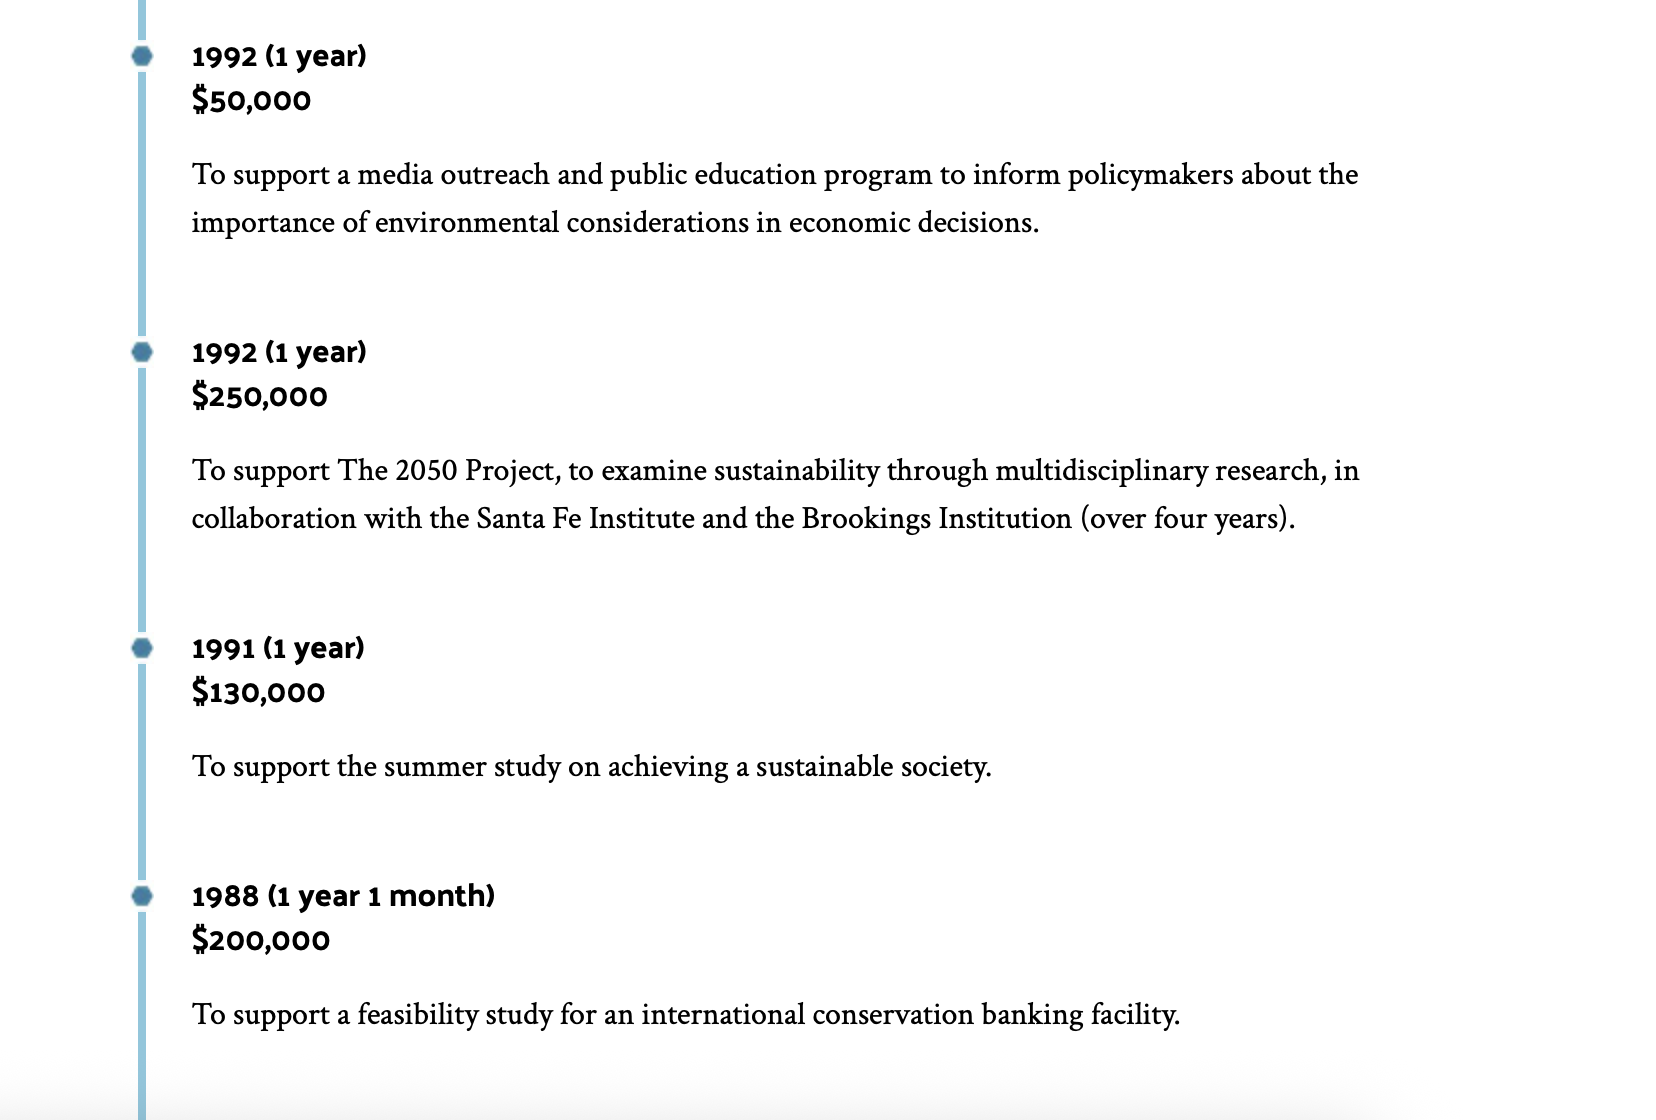
\includegraphics[width=0.8\textwidth]{figures/MacArthur_grants.png}
  \caption{Liste des financements accordés par la MacArthur Foundation sur son site internet}
  \label{fig:graph_grants_Project2050}
\end{figure}


Ce n’est que dans un second temps que certains projets bénéficient de subventions décisives. 

David Hendry explique dans son entretien avoir bénéficié du soutien de l’ESRC pour l’acquisition de son premier ordinateur personnel, et souligne que les financements de recherche en économétrie incluaient presque toujours une composante de développement logiciel, ce dernier étant indispensable à l’avancée de la discipline elle-même, étroitement liée à l’informatique (comme l’a également noté Renfro \cite{renfroEconometricsComputerLove2011} \cite{renfroEconometricSoftwareFirst2004}). Toutefois, aucun de ces financements n'est exclusivement consacré à la création et à la maintenance des logiciels : ils sont intégrés dans des projets de recherche plus larges, dont la programmation constitue une condition nécessaire mais non un objectif en soi.

La National Science Foundation (NSF) finance Gambit entre 1994 et 1999, permettant sa réécriture en C++ et une importante extension de ses fonctionnalités.

Mais si les financements sont déterminants pour le lancement, leur maintien en condition opérationnel, sur le long terme se révèle beaucoup plus difficile. En 1999, lorsque le financement de l’ESRC arrive à son terme, Pierse est poussé par l'institution à commercialiser le logiciel, car elle souhaite voir le logiciel maintenu. WinSolve est alors commercialisé par Timberlake Consultants, une entreprise spécialisée dans la distribution de logiciels dédiés à l'économétrie, la statistique et la prévision. 

La même incitation avait été faite à Hendry quelques années avant, rendant l'utilisation de PcGive payante. 

Gambit connaît un destin encore plus incertain : après la fin du soutien de la NSF, il survit près de vingt ans grâce au volontarisme de Turocy et de quelques collaborateurs, sans véritable financement structuré.  Et le développement du logiciel s’en trouve affecté, comme en témoigne Turocy dans son entretien et comme le montre ce graphique présentant le nombre d’additions et de suppressions de code réalisées dans Gambit au fil des années : on y observe une activité soutenue à la fin des années 1990 et au début des années 2000, suivie de phases de ralentissement, voire de quasi-abandon, avant une reprise en 2021. 

Cette évolution traduit bien le caractère irrégulier et dépendant des disponibilités individuelles du développement du logiciel, plutôt que le développement continu d’un projet durablement financé.

\begin{figure}[h]
  \centering
  \includegraphics[width=0.8\textwidth]{figures/code_frequency_Gambit.png}
  \caption{Évolution de l’activité de développement du logiciel Gambit (1995–2025)}
  \label{fig:graph_commits_Gambit}
\end{figure}

Quant à Sugarscape, le logiciel n'est pas maintenu après la publication des résultats du Project 2050 et du livre \cite{epsteinGrowingArtificialSocieties1996} : le logiciel laisse une trace durable dans la littérature, mais ne connait pas de développement actif. Le concept est cependant repris et développé dans de nombreux logiciels dont les plus connus sont NetLogo, MASON ou Repast.

Dans tous ces cas, la question de la pérennité financière apparaît comme un point de fragilité majeur.

À ces difficultés matérielles s’ajoute le problème de la faible reconnaissance académique. Plusieurs concepteurs soulignent combien il est difficile de publier des articles directement centrés sur le développement ou l’architecture de leurs logiciels. 

Pierse raconte avoir subi une certaine pression de la part de son employeur, l'Université de Surrey, pour limiter son temps de travail sur WinSolve. En effet, ce travail chronophage est quasiment impossible à transformer en publication, ou du moins les revues refuse ses soumissions sur WinSolve, quand bien même l’outil suscite un vif intérêt auprès de ses utilisateurs. 

De même, Fischbacher voit ses soumissions d'articles au journal \textit{Experimental Economics} rejetées, avant que ce même journal accepte de publier un article décrivant z-Tree en 2007, alors même que le logiciel était déjà devenu un standard de facto dans les laboratoires expérimentaux. Cette réticence des revues traduit un biais profond : la programmation est perçue comme un travail technique, auxiliaire de la recherche, et non comme une contribution scientifique en soi.

Le cas de Jurgen Doornik, qui est en charge de la plupart du travail technique sur PcGive et OxMetrics, est particulièrement éclairant : malgré ses contributions majeures — réécriture de l’ensemble des logiciels de David Hendry, création du langage Ox —, Pierse dans son entretien, estime qu'il n'a pas reçu la reconnaissance que mériterait un tel apport :

\begin{quote}
\begin{center}
\textit{"People who were spending a lot of time actually doing programming were not the people who were having great academic careers. I mean, that’s what I sort of observed. People like Jurgen Doornik, for example […] not really had the ... acclaim ... that I think he deserves. […] The top journals won’t ever publish stuff on this sort of thing"}
\end{center}
\end{quote} \hfill Déclaration de Pierse, page 25 de l'entretien pour Oral History of Economics \cite{pierseInterviewRichardPierse2024}



Fischbacher, pour tenter de pallier à cette faible reconnaissance, choisit dès 1997 de diffuser z-Tree sous la forme d’un \textit{citeware}. Ce type de licence impose que toute publication scientifique utilisant le logiciel mentionne explicitement son emploi et cite un article de référence dans la bibliographie. Dans le cas de z-Tree, cet article de référence demeure longtemps un working paper, à cause des difficultés mentionnées ci-dessus à faire publier son travail. Ce n’est qu’en 2007 que le journal Experimental Economics accepte de publier une version définitive, alors même que z-Tree s'est déjà un standard dans les laboratoires expérimentaux. Malgré ce décalage, le working paper commence à être cité massivement bien avant sa parution officielle :

\begin{figure}[h]
  \centering
  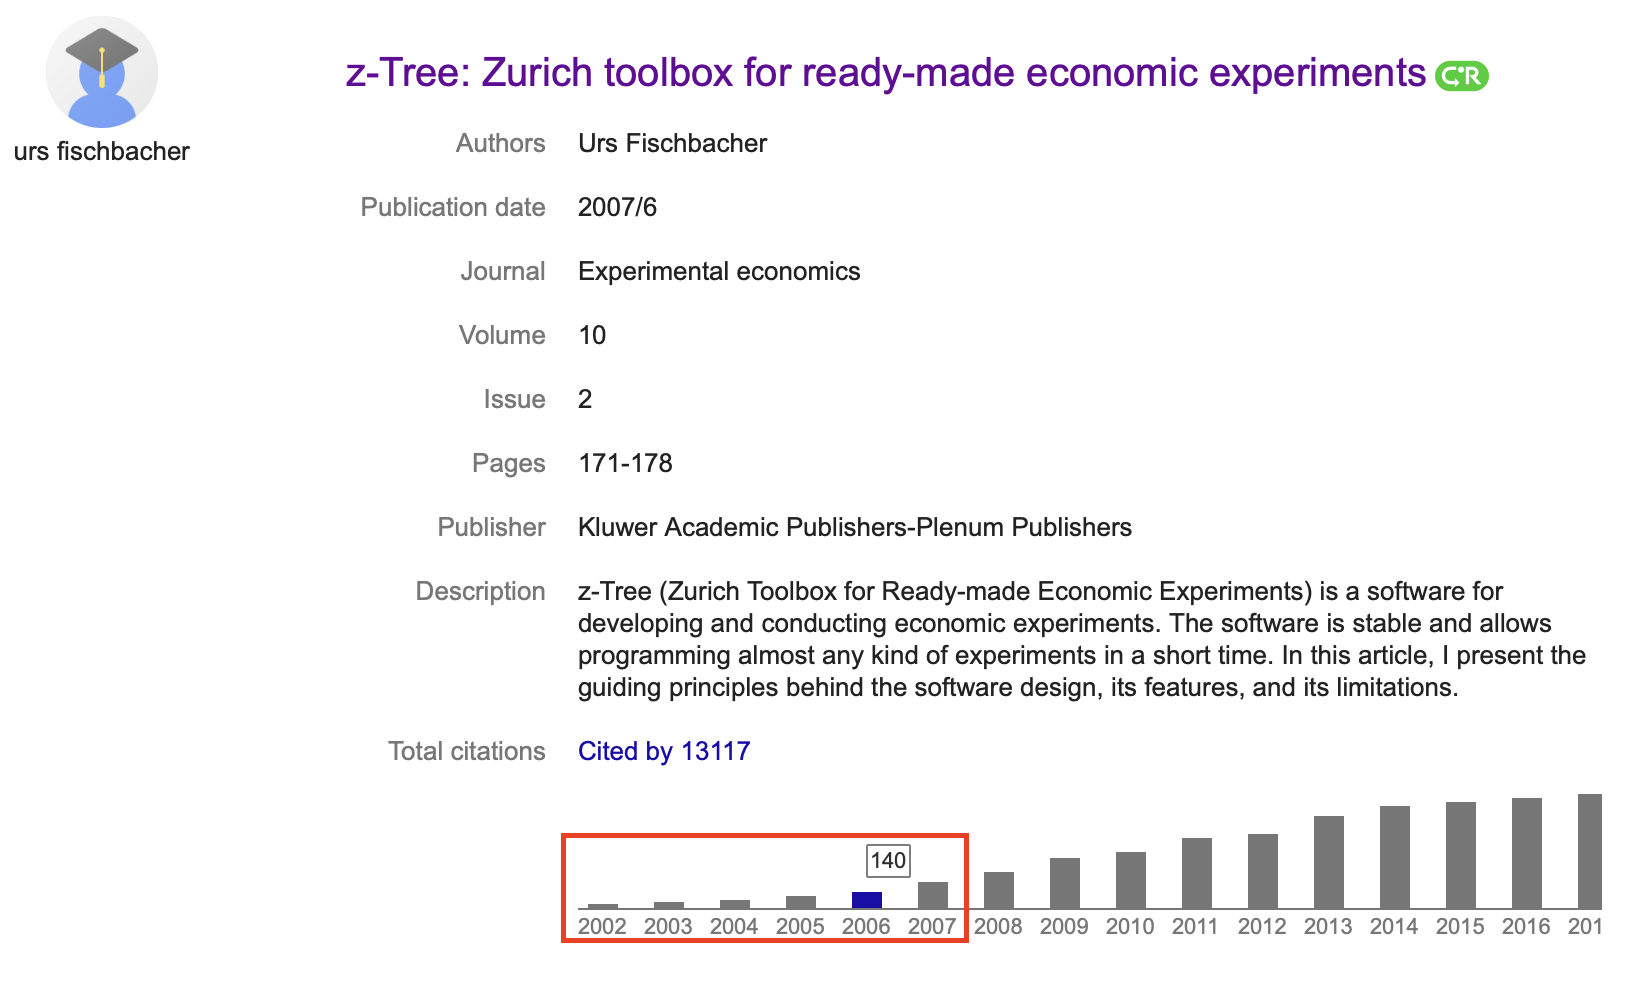
\includegraphics[width=0.8\textwidth]{figures/citation_z_tree.png}
  \caption{Nombre de citation par années de l'article de référence de z-Tree, source : Google Scholar}
  \label{fig:graph_citation_z_tree}
\end{figure}


Turocy, dit d'ailleurs dans son entretien\footnote{A la page 23}, s'être explicitement inspiré de Fischbacher et de ce modèle de \textit{citeware} pour Gambit. Ce qui permet à l'article de référence de cumuler plus de 600 citations en 2025, là aussi l'article le plus mentionné de Turocy.

L’article de référence sur z-Tree \cite{fischbacherz-TreeZurichToolbox2007} cumule ainsi, en 2025, plus de 13 000 citations, ce qui en fait de très loin la publication la plus citée d’Urs Fischbacher. Si le nombre de citations est souvent décrié par la communauté scientifique pour évaluer l'impact d'un article de recherche, une telle ampleur a nécessairement renforcé la visibilité et la reconnaissance de son auteur : c’est bien son travail de programmation qui se trouve ici crédité et valorisé.
Théodore Turocy explique d’ailleurs dans son entretien\footnote{Entretien avec Turocy\cite{turocyInterviewTheodoreTurocy2024}, p. 23} s’être explicitement inspiré de Fischbacher et de ce modèle de \textit{citeware} pour Gambit. L’article de référence du logiciel cumule ainsi, en 2025, plus de 600 citations — devenant aussi la publication la plus citée de Turocy. Ce parallèle montre combien le dispositif de \textit{citeware} constitue une stratégie efficace pour transformer un travail de programmation, difficile à valoriser, en une contribution reconnue dans le champ académique.

En somme, l’histoire de ces logiciels met en évidence un décalage structurel : bien qu’ils constituent des instruments essentiels pour certains domaines de la recherche en économie, ils peinent à être pleinement reconnu auprès des institutions. Leur émergence dépend souvent d’initiatives individuelles ou de financements circonstanciels, et leur maintien repose sur le volontarisme de leurs concepteurs, plus que sur des dispositifs pérennes. Financièrement, ils sont fragilisés par la dépendance à des subventions temporaires ou à des arrangements ad hoc difficiles à prolonger ; académiquement, ils souffrent d’un manque de reconnaissance, la programmation étant encore perçue comme une activité technique et secondaire, en marge de la "vraie" production scientifique que seraient les articles théoriques ou empiriques. Cette double contrainte, précarité matérielle et faible valorisation académique, contribue à expliquer pourquoi certains logiciels, pourtant centraux dans la transformation des pratiques économiques, peinent à s’inscrire durablement dans l’histoire officielle de la discipline.




\section{Postérité et devenir des logiciels}


La postérité des logiciels étudiés est contrastée. Certains continuent d’être diffusés et utilisés, d’autres ne subsistent plus qu’à travers leur rôle fondateur dans la littérature, et d’autres encore connaissent un maintien limité grâce à l’engagement de leurs concepteurs.

La suite logicielle issue de PcGive, développée par David Hendry et Jurgen Doornik, continue d’être diffusée commercialement par Timberlake Consultants en 2025. La dernière mise à jour date de juin 2024 (version 9.3), comme l’indique le site de Jurgen Doornik\url{https://www.doornik.com}. Une conférence des usagers d’OxMetrics s’est également tenue à Oxford les 3 et 4 avril 2025, toujours selon cette source. Elle demeure encore utilisée et mentionnée dans certains articles de recherches publiés par Hendry et Doornik\cite{castleSelectingModelForecasting2021} \cite{castleDetectingBreaksTrends2025}, en particulier en économétrie des séries temporelles. Toutefois, son statut de quasi-standard des années 1990 est progressivement concurrencé par des logiciels plus largement adoptés. Il reste difficile d’évaluer le nombre d’utilisateurs actifs en 2025, mais un constat ressort des recherches effectuées : aucun programme d’enseignement de l'économétrie récent (au cours des deux ou trois dernières années) dans les grandes universités occidentales ne fait mention de PcGive ou d’OxMetrics. Cette absence dans la formation initiale suggère que la communauté d’utilisateurs se réduit, en contraste avec la large diffusion de logiciels concurrents comme SAS, Stata, EViews ou R.

WinSolve connait un destin plus limité. La dernière version stable (4.0) date de 2007. Dans son entretien, Richard Pierse indique avoir continué à intervenir ponctuellement sur le code jusqu’en 2021, mais le logiciel n’est plus véritablement maintenu depuis. Il est utilisé pendant un temps dans certaines banques centrales et laboratoires, mais ne réussi pas à s’imposer durablement face à des environnements de modélisation macroéconomique plus flexibles comme Dynare. Sa trajectoire illustre la difficulté des logiciels dépendant d’un individu isolé à se maintenir dans le temps.

z-Tree constitue l’un des cas les plus durables. Il est conçu en 1995 et diffusé à l’international dès la fin des années 1990, il s'impose comme le standard de l’économie expérimentale. Sa robustesse et sa simplicité d’utilisation expliquent ce succès, mais il est aujourd’hui concurrencé par de nouvelles solutions, plus adaptées à l'ère du numérique. O-tree, une plateforme open source basée sur le web, est l'alternative la plus notable, car elle permet de mener des expériences en ligne et de configurer les expériences en utilisant le langage Python, bien plus connu et répandu que le langage z-Tree, spécifique à ce logiciel. D'autres variantes, comme z-Tree Unleashed, cherchent à prolonger l'outil original en repoussant ses limites techniques via le web. Bien que z-Tree conserve une position solide dans les laboratoires, son règne est désormais contesté par ces nouvelles solutions, qu'il a inspiré, conçues pour l'expérimentation en ligne.


Après avoir survécu de longues années grâce au volontarisme de Theodore Turocy, Gambit connaît aujourd’hui un renouveau partiel grâce à son intégration dans le projet "Automated analysis of strategic interactions" financé par l’Alan Turing Institute, notamment dans le domaine de l’intelligence artificielle et des agents autonomes. Son usage en économie reste limité, mais sa pertinence pour la modélisation computationnelle des agents lui confère une seconde vie, désormais plus souvent dans les cercles académiques de la théorie des jeux appliquée à d'autres disciplines que l'économie.


Sugarscape laisse une empreinte intellectuelle considérable, mais son existence logicielle est éphémère. Développé sur Macintosh, il est resté peu diffusé à l’époque, utilisé presque exclusivement par Epstein et Axtell. Après la publication de Growing Artificial Societies en 1996, le logiciel n’est pas maintenu, mais son influence se prolonge par la diffusion de la méthode de simulation multi-agents. Plusieurs environnements reprennent ses principes, notamment NetLogo, qui permet de reproduire les modèles originaux (comme celui des chasseurs-cueilleurs décrit par Epstein et Axtell), ainsi que MASON et Repast. Sugarscape est plus cité qu’utilisé : son importance tient à son rôle séminal dans l’ABM plutôt qu’à une trajectoire propre comme logiciel.


Ces différents destins soulignent que la postérité d’un logiciel ne dépend pas seulement de sa valeur scientifique initiale, mais aussi de son modèle de diffusion (open source ou commercial) et de sa capacité s’adapter aux évolutions techniques. Certains, comme Sugarscape, survivent comme références intellectuelles plus que comme outils utilisés ; d’autres, comme z-Tree ou OxMetrics, continuent à être employés mais sous la pression de la concurrence.\\





L’examen des logiciels développés par les programmeurs-économistes met en évidence un ensemble de traits communs et de contrastes qui permettent de mieux comprendre la place de l’informatique dans la discipline. Leur genèse répond presque toujours à un besoin local : faciliter l’enseignement de l’économétrie, résoudre des modèles macroéconomiques complexes, stabiliser des expériences de laboratoire ou encore explorer des phénomènes sociaux nouveaux à travers la simulation. Ces logiciels portent la marque de la débrouillardise et du pragmatisme de leurs concepteurs, qui bricolent avec les moyens techniques disponibles pour répondre à une contrainte immédiate.
Certains de ces outils ont ensuite dépassé leur fonction initiale pour devenir de véritables instruments heuristiques. Sugarscape et Gambit, en particulier, illustrent comment la simulation computationnelle peut ouvrir de nouveaux champs de recherche. Dans ces cas, la programmation ne se limite pas à exécuter des routines : elle devient une manière d’expérimenter, de découvrir et de reformuler les standards de l’explication économique.

Mais ces trajectoires sont traversées par des difficultés récurrentes. Le développement de logiciels confronte les chercheurs à des obstacles techniques lourds — choix des langages, contraintes de mémoire, conception d’interfaces ou stabilité des réseaux — qui exigent une expertise rarement valorisée par la discipline. Sur le plan institutionnel, les concepteurs se heurtent à la précarité du financement et à une reconnaissance académique limitée. Les revues hésitent à publier des articles centrés sur l’architecture logicielle, et les carrières des programmeurs-économistes pâtissent du temps consacré à ces tâches jugées « techniques ».

Enfin, l’analyse de la postérité de ces logiciels révèle des trajectoires contrastées. Certains, comme z-Tree ou PcGive/OxMetrics, se sont imposés comme des standards, tout en étant progressivement concurrencés par des alternatives. D’autres, comme WinSolve ou Gambit, ont connu une diffusion limitée ou intermittente, tributaires du volontarisme de leurs créateurs. D’autres encore, comme Sugarscape, ont davantage survécu comme références intellectuelles que comme instruments effectivement utilisés. Cette diversité des devenirs illustre la tension constante entre l’utilité pratique de ces logiciels, leur fragilité technique et leur faible reconnaissance institutionnelle.\\




Après avoir retracé l’histoire des logiciels conçus par les programmeurs-économistes et les difficultés récurrentes auxquelles ils se sont heurtés, la suite de ce travail portera sur l'analyse de leurs spécifités. Le chapitre suivant analysera plus particulièrement comment l'histoire de l'informatique et le contexte d'apprentissage de l'informatique ont produits de tels logiciels. Nous nous intéresserons ensuite à l'évolution des outils informatique de l'économiste qui permettent l'avénement d'économistes-programmeurs.

\chapter{Les constats et leçons à tirer}
\section{Des programmeurs-économistes forgés par les sciences "dures" et l’informatique rudimentaire, porteuses de logiciels ambitieux}

Les logiciels qui composent notre corpus naissent relativement tôt dans l'histoire et le développement de l'informatique moderne. PcGive de Hendry est conçu sur les premiers PC, à partir de programmes initialement écrits pour les ordinateurs mainframes. Ainsi, alors que l'informatique en tant qu'outil technique est en train d'être mise au point, la création de logiciels et l'informatisation de l'économie débute déjà.


Les entretiens analysés montrent un fait frappant : les créateurs de logiciels en économie ne sont pas formés en premier lieu comme économistes.

Ils viennent majoritairement des sciences dites "dures" ou "exactes" : mathématiques, informatique, ingénierie ou physique. Et il semble que cela soit également vrai au-delà de notre corpus, comme nous avons pu le voir avec les exemples de Dynare et OpenFisca.
Ce constat peu paraitre étonnant au premier abord, les logiciels produits par ces programmeurs sont tous destinés à la recherche en économie. Mais il n'a en fait rien de surprenant. L’informatique est historiquement issue des mathématiques, de la physique et de l’ingénierie comme l'explique Matti Tedre, historien et philosophe de l'informatique dans son livre \textit{"The Science of Computing: Shaping a Discipline"}\cite{tedreScienceComputingShaping2014}. De plus son enseignement a été, et reste aujourd’hui, institutionnellement rattaché à ces disciplines, alors que l’économie est classée parmi les sciences humaines et sociales.

À titre d'exemple, on peut constater que :
\begin{itemize}
  \item A l’université Paris 1, l’enseignement et la recherche en mathématique et informatique sont regroupés au sein de l’UFR 27, tandis que les sciences économiques forment l’UFR02.
  \item A l’université Paris Saclay, la licence d’économie est logée au sein de l’UFR de Droit, Économie et Gestion, tandis que la licence d’informatique se trouve au sein de la Faculté des sciences regroupant Mathématiques, Informatique, Physique, Chimie, Biologie et Sciences de la Terre.
  \item A la Sorbonne Université (fusion de Paris IV et Paris VI) l’informatique est logée dans la faculté des sciences et ingénierie, les Sciences humaines au sens large (pas de licence d’économie) sont regroupées dans la faculté des lettres.
  \item A Oxford, le département d'informatique appartient à la \textit{Mathematical, Physical and Life Sciences Division} tandis que celui d'économie appartient à la \textit{Social Sciences Division}
\end{itemize}

Il est donc normal que les premiers logiciels destinés à l’économie, que le processus d’informatisation de l’économie, ait été portée par des personnes issues d'autres disciplines. Mais ayant acquis, du fait de leurs parcours académique, des compétences poussées de programmation.

Ce découpage institutionnel reflète une division du travail : les compétences en programmation sont acquises ailleurs, et importées ensuite en économie. Il n’est donc pas étonnant que les premiers logiciels économiques aient été développés par des profils hybrides, programmeurs avant d’être économistes.



Ces trajectoires individuelles s’inscrivent toutes à une période où la programmation est encore une pratique nouvelle et en plein essor. Cette génération a donc appris à maitriser cette technologie dans un cadre rudimentaire.

Cette nouvelle technologie est alors porteuse de grandes promesses mais les contraintes matérielles sont encore lourdes. Les machines disposent de très peu de mémoire, beaucoup de logiciels ne disposent pas d'interfaces graphiques\footnote{Pour les utiliser, il faut alors utiliser une interface en ligne de commande (CLI). C'est le cas de PcGive dont on peut tester le fonctionnement sur le museum numérique de Jurgen Doornik: \url{https://museumofeconometrics.org.doornik.com/}}, et les langages de programmation restent rudimentaires (Fortran, Pascal, BASIC). L’apprentissage exige une compréhension profonde du fonctionnement des machines et l'utilisation de langage de bas niveau, produisant ainsi des programmeurs particulièrement à l’aise techniquement — bien plus que les générations suivantes, formées dans des environnements plus conviviaux. Une littérature journalistique et scientifique s'attache d'ailleurs à analyser ce phénomène de pertes de compétences des \textit{digital natives}. On peut citer à ce sujet cet article de Kirschner et De Bruyckere \cite{kirschnerMythsDigitalNative2017} et cet article de Georgia Wells dans le Wall Street Journal\cite{wellsGenZersAre2024}.

Ce constat rejoint un paradoxe bien documenté : contrairement à l’idée répandue du « digital native », l’exposition précoce aux technologies ne garantit ni compétence, ni autonomie critique. L’ICILS 2018 (International Computer and Information Literacy Study) montre par exemple que seuls 2\% des étudiants évalués atteignent le niveau le plus élevé de littératie numérique, c’est-à-dire la capacité à utiliser l’informatique de manière créative et critique pour produire de l’information nouvelle.

La majorité reste cantonnée à un usage élémentaire, et à peine 19\% des élèves sont capables d’utiliser les technologies de façon autonome pour rechercher, évaluer et gérer l’information \footnote{ICILS 2018, International Computer and Information Literacy Study, IEA, \url{https://www.iea.nl/studies/iea/icils/2018}}. Et ce phénomène touche aussi la population des programmeurs. Voilà ce que l'on peut lire dans le rapport de 2018 sur les compétences des développeurs publié par HackerRank\cite{2018DeveloperSkills} :

\begin{quote}
\begin{center}
\textit{"Unlike generations thereafter, if kids of the seventies wanted to see innovative technology, they’d have to build it themselves — they had no other choice. There were no widespread resources to teach them how to build software. Almost half of all developers (47\%) between the ages of 45 and 54 started coding before they were 16 years old. Meanwhile, developers between 18 and 24 today are the least likely to have started coding before 16 (only 20\%).
Developers between the ages of 45 and 54 were among the first to get their hands on relatively powerful PCs, like the Acorn Archimedes, TRS-80, Commodore 64, and Apple II. With limited to no access to formal education, young people in the PC Revolution had an unusually strong drive to learn to code on their own."}
\end{center}
\end{quote} \hfill Extrait du Developer Skills Report de 2018, HackerRank\cite{2018DeveloperSkills}

Ce contexte a donc favorisé un apprentissage exigeant mais formateur. Ceux qui ont traversé cette phase d’appropriation sont devenus particulièrement à l’aise avec l’outil informatique. Ils ont acquis une maîtrise profonde de la programmation, bien plus poussée que celle des générations suivantes, formées dans des environnements déjà stabilisés et “conviviaux”.



Cette double caractéristique des programmeurs-économistes, formation en sciences "dures" et apprentissage dans un environnement technique contraint, explique qu'ils aient pu créer des logiciels d’une grande complexité à une époque où il faut presque tout construire. D'ailleurs, dans plusieurs entretiens, les programmeurs-économistes témoignent avoir passé beaucoup de temps à résoudre des problèmes très techniques et très éloignés de l'aspect purement économique des logiciels mais apportant beaucoup de valeur à leurs logiciels. Axtell témoigne par exemple qu'en l'absence d'outils dédiés à la visualisation, Epstein et lui on investi plusieurs jours et plusieurs milliers de dollars dans du matériel d'accélération vidéo. 

Fischbacher, dans le cadre du développement de z-Tree a passé énormément de temps à intégrer des fonctionnalités de réseau pour permettre l’interaction en temps réel entre participants d’expériences. Les programmeurs de WinSolve et PcGive ont consacré une attention particulière aux interfaces graphiques pour rendre l’outil accessible aux utilisateurs. Agnès Gramain enfin, a dû réécrire elle-même des algorithmes de base d’économétrie, comme celui de maximisation de la vraisemblance \footnote{Page 5 de l'entretien \cite{gramainInterviewAgnesGramain2024}}, aujourd'hui préprogrammé et disponible sur tous les logiciels d'économétrie.

Ces témoignages illustrent combien la valeur de ces logiciels ne tient pas seulement à leur contenu économique, mais aussi à la capacité de leurs concepteurs à surmonter des obstacles techniques fondamentaux, en dotant leurs outils de fonctionnalités inédites qui ont largement conditionné leur adoption et leur pérennité.










\section{Le passage des programmeurs-économistes aux économistes-programmeurs}


Mais aujourd’hui, l’écosystème informatique des économistes a profondément changé. Il n’est plus nécessaire d'avoir une maîtrise poussée des langages de bas niveau. Les langages de haut niveau comme R ou Python offrent des environnements beaucoup plus faciles à prendre en main pour des économistes de formation, non formés à l'ingénierie logicielle.
De nombreuses bibliothèques de codes sont disponibles, offrant à l'économiste une boite à outils très développés et optimisés par des informaticiens de métier et la communauté des usagers. Ce temps de travail que l'économiste n'a pas à fournir pour créer ses outils informatique, il peut alors le consacrer aux tâches dans lesquels il a la plus grande valeur ajoutée : la modélisation économique, la production de résultats empiriques et l’élaboration de nouvelles méthodes adaptées aux questions de recherche de l'économie. L'existence d'économistes-programmeurs est rendue possible par ces nouveaux outils.

Cette évolution s’accompagne d’un changement dans la manière de créer des outils. Alors que les pionniers devaient concevoir des logiciels entiers, des interfaces entre ces logiciels et leurs utilisateurs, parfois même des langages, la tendance actuelle est de développer des bibliothèques spécialisées, constituées de quelques dizaines de fonctions, destinées à répondre à un problème précis. Ces bibliothèques s’intègrent dans de vastes écosystèmes open source comme CRAN pour R ou PyPI pour Python. Elles bénéficient de la relecture et de l’appui d’une large communauté, ce qui limite les risques de bogues et garantit une certaine standardisation. Ce déplacement réduit les risques que des oublis ou des erreurs, inhérents au développement logiciel, compromettent des résultats. Mais il pose désormais un autre défi : se distinguer dans une offre pléthorique de packages, non plus en luttant contre l’invisibilité, mais en gagnant en visibilité au sein d’un marché saturé d’outils.

Cette situation modifie le profil des développeurs de logiciel en économie aujourd'hui, qui se sont adapté à ces changements. Les économistes-programmeurs d’aujourd’hui sont avant tout des économistes, et non des programmeurs venus d'autres disciplines. Leur compétence première est l'économie, et la programmation est un instrument secondaire qui peut être mobilisé lorsque l'étude d'une question économique le commande.


Cette forte recomposition de l'écosystème informatique des économistes a eu lieu au cours des deux dernières décennies et tous les dévelopeurs-économistes de notre corpus sont donc trop anciens pour les avoir vécus (Turocy a soutenu son doctorat en 2001). Nous pensons donc qu'il serait pertinent d’élargir ce corpus en menant des entretiens avec des économistes-programmeurs plus jeunes. Clément de Chaisemartin, par exemple, qui a obtenu son doctorat en 2013, a développé plusieurs packages économétriques, disponibles sur les logiciels R et Stata, destinés à l’estimation d’effets de traitement hétérogènes et à l’évaluation de politiques publiques\footnote{Voir \url{https://github.com/chaisemartinPackages}}, et constitue à ce titre un profil particulièrement intéressant.
On pourrait également s’intéresser aux équipes de l’Institut des politiques publiques (IPP) travaillant sur le logiciel de microsimulation TAXIPP. L’étude de ces chercheurs et de leurs pratiques permettrait de mieux comprendre comment la microsimulation, technique intrinsèquement liée à l’informatique, contribue à renforcer (ou non) le rôle de « conseiller du prince » des économistes. En effet, cette méthode s’est imposée au cœur des administrations françaises et y occupe une place très importante. Elle est notamment utilisée pour anticiper l’évolution des recettes et des dépenses liée aux impôts, taxes, cotisations et prestations de sécurité sociale.










\section{Toujours à la frontière de l'innovation, entre promesses et risques d’abstraction}


Un autre élément qui ressort de notre enquête est le sentiment permanent, partagé entre les générations de programmeurs-économistes, d’évoluer à la frontière de l’innovation. Comme l’écrit Renfro dans son article rétrospectif de 2004, \textit{Econometric Software: The first Fifty Years in Perspective} \cite{renfroEconometricSoftwareFirst2004}, 

\begin{quote}
\begin{center}
\textit{"The period of development of econometric software spans the professional careers of almost all working economists. At each step along the road, what constituted “the present” at that time seemed to offer both promise and the sense of being at the forefront.”}
\end{center}
\end{quote} \hfill \textit{Econometric Software: The first Fifty Years in Perspective}, page 58 \cite{renfroEconometricSoftwareFirst2004}

 
Cette impression était déjà présente dans les années 1970, lorsque la programmation se faisait sur des ordinateurs centraux ou sur des premiers PC encore balbutiants. Elle demeure aujourd’hui, même si l’environnement a radicalement changé : à chaque époque, l’informatisation de l’économie s’accompagne de l’idée que l’on se trouve à l’avant-garde technologique.

Les développements récents des grands modèles de langage (LLM) accentuent encore cette dynamique. Après être passés des langages bas niveau (Fortran, Cobol) aux langages de haut niveau (R, Python), les économistes peuvent désormais interagir avec la machine dans un langage proche du langage naturel. Les environnements de “vibe coding” ou l’usage de copilotes de programmation basés sur l’IA promettent d’abaisser encore la barrière technique. La génération actuelle dispose ainsi d’outils qui rendent la programmation plus accessible que jamais, au prix d’un éloignement toujours plus grand de la couche technique. Là où Hendry, Gramain ou Axtell devaient comprendre les algorithmes en profondeur, leurs successeurs peuvent aujourd’hui obtenir du code fonctionnel à partir d’une simple instruction en langage courant.

Mais cette nouvelle couche d’abstraction ne va pas sans risques. D’une part, les technologies d’intelligence artificielle appliquées à la programmation sont encore immatures, et leur fiabilité reste incertaine. D’autre part, elles renforcent une inquiétude déjà exprimée par Johnston il y a 45 ans et rappelée par Renfro dans son article de 2004 : celle d’une utilisation aveugle d’outils puissants, sans réelle compréhension de leurs fondements. Comme Johnston le soulignait en 1991, 


\begin{quote}
\begin{center}
\textit{“It is thus all too possible for someone to activate an econometric software package, of which he has only a dim understanding, to apply it to data of whose nature and provenance he is ignorant, and then to draw conclusions about an economic situation, whose historical and institutional realities he has, perhaps, not studied in any depth.”}
\end{center}
\end{quote} \hfill \textit{Econometrics Retrospect and Prospect }, page 2 \cite{johnstonEconometricsRetrospectProspect1991}


Le danger est bien celui d’une déconnexion entre l’économiste et les données, entre l’utilisateur et l’outil. L’innovation technologique, en offrant des solutions de plus en plus “clé en main”, facilite l’accès à l’informatique mais peut aussi fragiliser la capacité critique de ceux qui s’en servent.




\chapter*{Conclusion}
\addcontentsline{toc}{chapter}{Conclusion}

Ce mémoire avait pour objectif d’analyser la place des logiciels dans la pratique économique, à travers l’étude de 7 entretiens réalisés avec des programmeurs-économistes. L’ambition était double : documenter un pan encore peu exploré de l’histoire récente de l’économie et proposer une analyse de l’informatisation de la discipline. Le recours à la méthode de l'histoire orale a été indispensable pour pemettre de saisir non seulement des trajectoires individuelles, mais aussi la manière dont les chercheurs eux-mêmes décrivent leurs rapports à l’informatique, à l'économie, aux langages de programmation et aux outils qu’ils ont contribué à développer. En effet, comme nous l'avons vu dans ce mémoire, ces pratiques transparaissent peu dans la littérature académique, du fait d'un manque de légitimité de celles-ci auprès des principaux journaux.

L’analyse de ces témoignages met en évidence plusieurs résultats. Tout d’abord, l’informatisation de l’économie est portée par des chercheurs souvent issus des sciences dites « dures » (mathématiques, informatique, ingénierie, physique) et formés à la programmation qui s'intéressent à l'économie dans un second temps et y importent leurs compétences techniques. Cette hybridité disciplinaire a joué un rôle déterminant dans la capacité à créer des logiciels robustes et complexes à une époque où l’informatique restait instable et rudimentaire. Ensuite, le développement de ces outils précurseurs s’est accompagné d’un travail considérable d’ingénierie logicielle, bien au-delà de la seule dimension économique. Enfin, l’évolution récente des environnements informatiques a profondément transformé la pratique : l’essor des langages de haut niveau et des écosystèmes open source (R, Python) permet désormais aux économistes d’utiliser et de produire des outils sans avoir à réinventer les fondations logicielles. Ces innovations technologiques permettent aujourd'hui l'avènement d'économistes-programmeurs, se définissant d’abord comme économistes, et seulement ensuite comme programmeurs.

Au-delà de ces constats empiriques, cette enquête conduit à une réflexion plus générale sur la dynamique de l’informatisation de l’économie. Trois leçons principales se dégagent.

Premièrement, l’économie s’inspire abondamment des sciences dures pour se développer, mais cette appropriation ne concerne pas uniquement des compétences techniques (programmation, simulation), elle s'étend aussi aux cadres conceptuels. Comme l’ont analysé Mirowski dans \textit{Machine Dreams : Economics Becomes a Cyborg Science}\cite{mirowskiMachineDreamsEconomics2001} et \textit{More Heat than Light : Economics as Social Physics, Physics as Nature's Economics}\cite{mirowskiMoreHeatLight1989} et McCloskey dans \textit{the rethoric of Economics}\cite{mccloskeyRhetoricEconomics1983}, l’économie a une longue tradition d’emprunt aux mathématiques, à la physique ou à la biologie, pour construire des métaphores et des analogies qui structurent ses modèles. 

Deuxièmement, cette ouverture permanente se combine, paradoxalement, à une inertie marquée dans certaines pratiques. Comme en témoigne Agnès Gramain dans son entretien, certains enseignants, dont elle fait partie, ont du mal à se défaire des logiciels propriétaires comme Stata ou SAS. Ces logiciels continuent d’occuper une place importante, non en raison de leurs performances, mais parce que les enseignants y sont habitués et continuent de les transmettre lors de leurs enseignements. Cette inertie institutionnelle limite la diffusion des outils open source comme R et Python.

Troisièmement, les programmeurs-économistes, dans leurs entretiens, confirment une forme de conservatisme générationnel, résumé par le principe de Planck : dans l’économie comme dans d’autres disciplines, les véritables changements ne s’imposent qu’avec le renouvellement des cohortes de chercheurs, “un décès à la fois”. L’économie apparaît donc à la fois comme une discipline ouverte, nourrie par les sciences "dures" et leurs métaphores, et comme une discipline résistante au changement, où l’innovation technologique et logicielle se heurte à des routines et à une adoption lente de la part des chercheurs les plus anciens.

Ce travail présente cependant plusieurs limites. Le corpus d’entretiens reste restreint et centré sur une génération de programmeurs ayant soutenu leurs thèses et produit leurs logiciels entre les années 1970 et 2000. Les trajectoires plus récentes, par exemple celles de développeurs de packages contemporains comme Clément de Chaisemartin ou des équipes de microsimulation de l’IPP, mériteraient d’être étudiées pour mieux comprendre comment les jeunes générations mobilisent les outils informatiques modernes de l'économiste. Par ailleurs, les entretiens, par nature, donnent accès à des récits situés et subjectifs. Ces limites de la méthode de l'histoire orale sont donc à garder à l'esprit.

L’étude de la microsimulation, technique intrinsèquement liée à l’informatique et désormais centrale dans l’expertise économique des politiques publiques, permettrait par exemple d’élargir la réflexion sur le rôle de l’informatique dans la construction de la figure de l'expert économique. De même, l’arrivée des grands modèles de langage (LLM) et des assistants de programmation automatisés invite à s’interroger sur les nouvelles couches d’abstraction qui transforment l’accès à la programmation et, potentiellement, le rapport des économistes à leurs outils.

En définitive, l’informatisation de l’économie n’apparaît pas comme un simple ajout d’outils à une discipline déjà constituée, mais comme une transformation profonde des manières de travailler, de modéliser et d’enseigner. Elle révèle une tension permanente : celle d’une discipline toujours à la frontière de l’innovation, mais en même temps freinée par ses routines et son conservatisme.

% \printglossary


%----------------------------------------------------------------------------------------
%	BIBLIOGRAPHY
%----------------------------------------------------------------------------------------
\printbibliography
%\nocite{*} % <-- if you want uncited entries, otherwise comment this out


\end{document}